% Created by tikzDevice version 0.11 on 2018-08-04 20:39:07
% !TEX encoding = UTF-8 Unicode
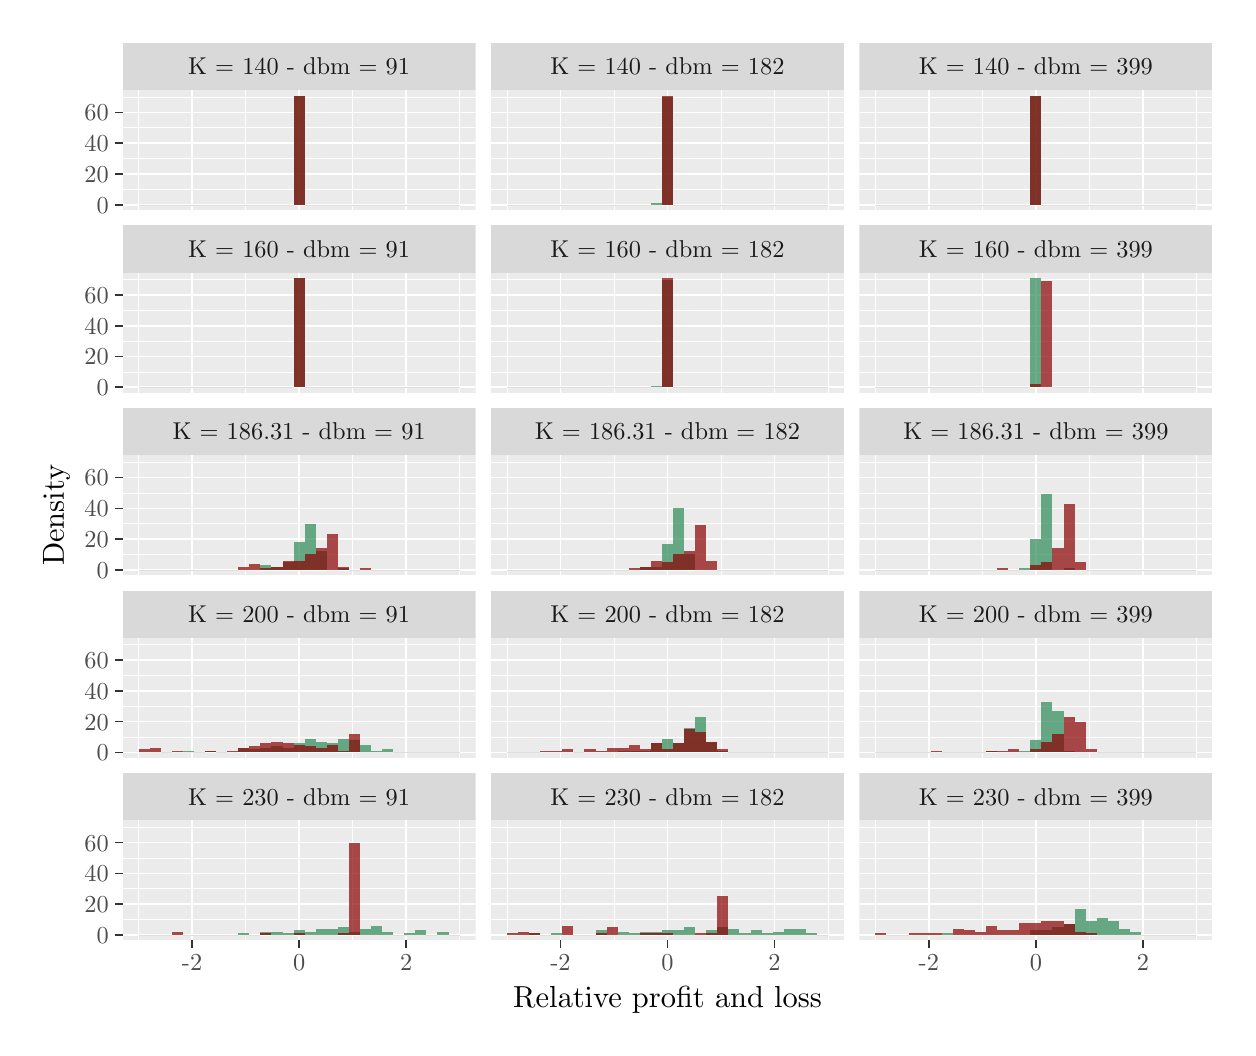
\begin{tikzpicture}[x=1pt,y=1pt]
\definecolor{fillColor}{RGB}{255,255,255}
\path[use as bounding box,fill=fillColor,fill opacity=0.00] (0,0) rectangle (433.62,361.35);
\begin{scope}
\path[clip] (  0.00,  0.00) rectangle (433.62,361.35);
\definecolor{drawColor}{RGB}{255,255,255}
\definecolor{fillColor}{RGB}{255,255,255}

\path[draw=drawColor,line width= 0.6pt,line join=round,line cap=round,fill=fillColor] (  0.00,  0.00) rectangle (433.62,361.35);
\end{scope}
\begin{scope}
\path[clip] ( 34.27,295.39) rectangle (161.89,338.79);
\definecolor{fillColor}{gray}{0.92}

\path[fill=fillColor] ( 34.27,295.39) rectangle (161.89,338.79);
\definecolor{drawColor}{RGB}{255,255,255}

\path[draw=drawColor,line width= 0.3pt,line join=round] ( 34.27,302.92) --
	(161.89,302.92);

\path[draw=drawColor,line width= 0.3pt,line join=round] ( 34.27,314.03) --
	(161.89,314.03);

\path[draw=drawColor,line width= 0.3pt,line join=round] ( 34.27,325.15) --
	(161.89,325.15);

\path[draw=drawColor,line width= 0.3pt,line join=round] ( 34.27,336.26) --
	(161.89,336.26);

\path[draw=drawColor,line width= 0.3pt,line join=round] ( 40.07,295.39) --
	( 40.07,338.79);

\path[draw=drawColor,line width= 0.3pt,line join=round] ( 78.74,295.39) --
	( 78.74,338.79);

\path[draw=drawColor,line width= 0.3pt,line join=round] (117.41,295.39) --
	(117.41,338.79);

\path[draw=drawColor,line width= 0.3pt,line join=round] (156.08,295.39) --
	(156.08,338.79);

\path[draw=drawColor,line width= 0.6pt,line join=round] ( 34.27,297.36) --
	(161.89,297.36);

\path[draw=drawColor,line width= 0.6pt,line join=round] ( 34.27,308.47) --
	(161.89,308.47);

\path[draw=drawColor,line width= 0.6pt,line join=round] ( 34.27,319.59) --
	(161.89,319.59);

\path[draw=drawColor,line width= 0.6pt,line join=round] ( 34.27,330.70) --
	(161.89,330.70);

\path[draw=drawColor,line width= 0.6pt,line join=round] ( 59.40,295.39) --
	( 59.40,338.79);

\path[draw=drawColor,line width= 0.6pt,line join=round] ( 98.08,295.39) --
	( 98.08,338.79);

\path[draw=drawColor,line width= 0.6pt,line join=round] (136.75,295.39) --
	(136.75,338.79);
\definecolor{fillColor}{RGB}{46,139,87}

\path[fill=fillColor,fill opacity=0.70] ( 40.07,297.36) rectangle ( 44.07,297.36);

\path[fill=fillColor,fill opacity=0.70] ( 44.07,297.36) rectangle ( 48.07,297.36);

\path[fill=fillColor,fill opacity=0.70] ( 48.07,297.36) rectangle ( 52.07,297.36);

\path[fill=fillColor,fill opacity=0.70] ( 52.07,297.36) rectangle ( 56.07,297.36);

\path[fill=fillColor,fill opacity=0.70] ( 56.07,297.36) rectangle ( 60.07,297.36);

\path[fill=fillColor,fill opacity=0.70] ( 60.07,297.36) rectangle ( 64.07,297.36);

\path[fill=fillColor,fill opacity=0.70] ( 64.07,297.36) rectangle ( 68.07,297.36);

\path[fill=fillColor,fill opacity=0.70] ( 68.07,297.36) rectangle ( 72.07,297.36);

\path[fill=fillColor,fill opacity=0.70] ( 72.07,297.36) rectangle ( 76.07,297.36);

\path[fill=fillColor,fill opacity=0.70] ( 76.07,297.36) rectangle ( 80.07,297.36);

\path[fill=fillColor,fill opacity=0.70] ( 80.07,297.36) rectangle ( 84.07,297.36);

\path[fill=fillColor,fill opacity=0.70] ( 84.07,297.36) rectangle ( 88.08,297.36);

\path[fill=fillColor,fill opacity=0.70] ( 88.08,297.36) rectangle ( 92.08,297.36);

\path[fill=fillColor,fill opacity=0.70] ( 92.08,297.36) rectangle ( 96.08,297.36);

\path[fill=fillColor,fill opacity=0.70] ( 96.08,297.36) rectangle (100.08,336.82);

\path[fill=fillColor,fill opacity=0.70] (100.08,297.36) rectangle (104.08,297.36);

\path[fill=fillColor,fill opacity=0.70] (104.08,297.36) rectangle (108.08,297.36);

\path[fill=fillColor,fill opacity=0.70] (108.08,297.36) rectangle (112.08,297.36);

\path[fill=fillColor,fill opacity=0.70] (112.08,297.36) rectangle (116.08,297.36);

\path[fill=fillColor,fill opacity=0.70] (116.08,297.36) rectangle (120.08,297.36);

\path[fill=fillColor,fill opacity=0.70] (120.08,297.36) rectangle (124.08,297.36);

\path[fill=fillColor,fill opacity=0.70] (124.08,297.36) rectangle (128.08,297.36);

\path[fill=fillColor,fill opacity=0.70] (128.08,297.36) rectangle (132.08,297.36);

\path[fill=fillColor,fill opacity=0.70] (132.08,297.36) rectangle (136.08,297.36);

\path[fill=fillColor,fill opacity=0.70] (136.08,297.36) rectangle (140.08,297.36);

\path[fill=fillColor,fill opacity=0.70] (140.08,297.36) rectangle (144.08,297.36);

\path[fill=fillColor,fill opacity=0.70] (144.08,297.36) rectangle (148.08,297.36);

\path[fill=fillColor,fill opacity=0.70] (148.08,297.36) rectangle (152.08,297.36);

\path[fill=fillColor,fill opacity=0.70] (152.08,297.36) rectangle (156.08,297.36);
\definecolor{fillColor}{RGB}{139,0,0}

\path[fill=fillColor,fill opacity=0.70] ( 40.07,297.36) rectangle ( 44.07,297.36);

\path[fill=fillColor,fill opacity=0.70] ( 44.07,297.36) rectangle ( 48.07,297.36);

\path[fill=fillColor,fill opacity=0.70] ( 48.07,297.36) rectangle ( 52.07,297.36);

\path[fill=fillColor,fill opacity=0.70] ( 52.07,297.36) rectangle ( 56.07,297.36);

\path[fill=fillColor,fill opacity=0.70] ( 56.07,297.36) rectangle ( 60.07,297.36);

\path[fill=fillColor,fill opacity=0.70] ( 60.07,297.36) rectangle ( 64.07,297.36);

\path[fill=fillColor,fill opacity=0.70] ( 64.07,297.36) rectangle ( 68.07,297.36);

\path[fill=fillColor,fill opacity=0.70] ( 68.07,297.36) rectangle ( 72.07,297.36);

\path[fill=fillColor,fill opacity=0.70] ( 72.07,297.36) rectangle ( 76.07,297.36);

\path[fill=fillColor,fill opacity=0.70] ( 76.07,297.36) rectangle ( 80.07,297.36);

\path[fill=fillColor,fill opacity=0.70] ( 80.07,297.36) rectangle ( 84.07,297.36);

\path[fill=fillColor,fill opacity=0.70] ( 84.07,297.36) rectangle ( 88.08,297.36);

\path[fill=fillColor,fill opacity=0.70] ( 88.08,297.36) rectangle ( 92.08,297.36);

\path[fill=fillColor,fill opacity=0.70] ( 92.08,297.36) rectangle ( 96.08,297.36);

\path[fill=fillColor,fill opacity=0.70] ( 96.08,297.36) rectangle (100.08,336.82);

\path[fill=fillColor,fill opacity=0.70] (100.08,297.36) rectangle (104.08,297.36);

\path[fill=fillColor,fill opacity=0.70] (104.08,297.36) rectangle (108.08,297.36);

\path[fill=fillColor,fill opacity=0.70] (108.08,297.36) rectangle (112.08,297.36);

\path[fill=fillColor,fill opacity=0.70] (112.08,297.36) rectangle (116.08,297.36);

\path[fill=fillColor,fill opacity=0.70] (116.08,297.36) rectangle (120.08,297.36);

\path[fill=fillColor,fill opacity=0.70] (120.08,297.36) rectangle (124.08,297.36);

\path[fill=fillColor,fill opacity=0.70] (124.08,297.36) rectangle (128.08,297.36);

\path[fill=fillColor,fill opacity=0.70] (128.08,297.36) rectangle (132.08,297.36);

\path[fill=fillColor,fill opacity=0.70] (132.08,297.36) rectangle (136.08,297.36);

\path[fill=fillColor,fill opacity=0.70] (136.08,297.36) rectangle (140.08,297.36);

\path[fill=fillColor,fill opacity=0.70] (140.08,297.36) rectangle (144.08,297.36);

\path[fill=fillColor,fill opacity=0.70] (144.08,297.36) rectangle (148.08,297.36);

\path[fill=fillColor,fill opacity=0.70] (148.08,297.36) rectangle (152.08,297.36);

\path[fill=fillColor,fill opacity=0.70] (152.08,297.36) rectangle (156.08,297.36);
\end{scope}
\begin{scope}
\path[clip] ( 34.27,229.42) rectangle (161.89,272.83);
\definecolor{fillColor}{gray}{0.92}

\path[fill=fillColor] ( 34.27,229.42) rectangle (161.89,272.83);
\definecolor{drawColor}{RGB}{255,255,255}

\path[draw=drawColor,line width= 0.3pt,line join=round] ( 34.27,236.95) --
	(161.89,236.95);

\path[draw=drawColor,line width= 0.3pt,line join=round] ( 34.27,248.07) --
	(161.89,248.07);

\path[draw=drawColor,line width= 0.3pt,line join=round] ( 34.27,259.18) --
	(161.89,259.18);

\path[draw=drawColor,line width= 0.3pt,line join=round] ( 34.27,270.30) --
	(161.89,270.30);

\path[draw=drawColor,line width= 0.3pt,line join=round] ( 40.07,229.42) --
	( 40.07,272.83);

\path[draw=drawColor,line width= 0.3pt,line join=round] ( 78.74,229.42) --
	( 78.74,272.83);

\path[draw=drawColor,line width= 0.3pt,line join=round] (117.41,229.42) --
	(117.41,272.83);

\path[draw=drawColor,line width= 0.3pt,line join=round] (156.08,229.42) --
	(156.08,272.83);

\path[draw=drawColor,line width= 0.6pt,line join=round] ( 34.27,231.40) --
	(161.89,231.40);

\path[draw=drawColor,line width= 0.6pt,line join=round] ( 34.27,242.51) --
	(161.89,242.51);

\path[draw=drawColor,line width= 0.6pt,line join=round] ( 34.27,253.62) --
	(161.89,253.62);

\path[draw=drawColor,line width= 0.6pt,line join=round] ( 34.27,264.74) --
	(161.89,264.74);

\path[draw=drawColor,line width= 0.6pt,line join=round] ( 59.40,229.42) --
	( 59.40,272.83);

\path[draw=drawColor,line width= 0.6pt,line join=round] ( 98.08,229.42) --
	( 98.08,272.83);

\path[draw=drawColor,line width= 0.6pt,line join=round] (136.75,229.42) --
	(136.75,272.83);
\definecolor{fillColor}{RGB}{46,139,87}

\path[fill=fillColor,fill opacity=0.70] ( 40.07,231.40) rectangle ( 44.07,231.40);

\path[fill=fillColor,fill opacity=0.70] ( 44.07,231.40) rectangle ( 48.07,231.40);

\path[fill=fillColor,fill opacity=0.70] ( 48.07,231.40) rectangle ( 52.07,231.40);

\path[fill=fillColor,fill opacity=0.70] ( 52.07,231.40) rectangle ( 56.07,231.40);

\path[fill=fillColor,fill opacity=0.70] ( 56.07,231.40) rectangle ( 60.07,231.40);

\path[fill=fillColor,fill opacity=0.70] ( 60.07,231.40) rectangle ( 64.07,231.40);

\path[fill=fillColor,fill opacity=0.70] ( 64.07,231.40) rectangle ( 68.07,231.40);

\path[fill=fillColor,fill opacity=0.70] ( 68.07,231.40) rectangle ( 72.07,231.40);

\path[fill=fillColor,fill opacity=0.70] ( 72.07,231.40) rectangle ( 76.07,231.40);

\path[fill=fillColor,fill opacity=0.70] ( 76.07,231.40) rectangle ( 80.07,231.40);

\path[fill=fillColor,fill opacity=0.70] ( 80.07,231.40) rectangle ( 84.07,231.40);

\path[fill=fillColor,fill opacity=0.70] ( 84.07,231.40) rectangle ( 88.08,231.40);

\path[fill=fillColor,fill opacity=0.70] ( 88.08,231.40) rectangle ( 92.08,231.40);

\path[fill=fillColor,fill opacity=0.70] ( 92.08,231.40) rectangle ( 96.08,231.40);

\path[fill=fillColor,fill opacity=0.70] ( 96.08,231.40) rectangle (100.08,270.85);

\path[fill=fillColor,fill opacity=0.70] (100.08,231.40) rectangle (104.08,231.40);

\path[fill=fillColor,fill opacity=0.70] (104.08,231.40) rectangle (108.08,231.40);

\path[fill=fillColor,fill opacity=0.70] (108.08,231.40) rectangle (112.08,231.40);

\path[fill=fillColor,fill opacity=0.70] (112.08,231.40) rectangle (116.08,231.40);

\path[fill=fillColor,fill opacity=0.70] (116.08,231.40) rectangle (120.08,231.40);

\path[fill=fillColor,fill opacity=0.70] (120.08,231.40) rectangle (124.08,231.40);

\path[fill=fillColor,fill opacity=0.70] (124.08,231.40) rectangle (128.08,231.40);

\path[fill=fillColor,fill opacity=0.70] (128.08,231.40) rectangle (132.08,231.40);

\path[fill=fillColor,fill opacity=0.70] (132.08,231.40) rectangle (136.08,231.40);

\path[fill=fillColor,fill opacity=0.70] (136.08,231.40) rectangle (140.08,231.40);

\path[fill=fillColor,fill opacity=0.70] (140.08,231.40) rectangle (144.08,231.40);

\path[fill=fillColor,fill opacity=0.70] (144.08,231.40) rectangle (148.08,231.40);

\path[fill=fillColor,fill opacity=0.70] (148.08,231.40) rectangle (152.08,231.40);

\path[fill=fillColor,fill opacity=0.70] (152.08,231.40) rectangle (156.08,231.40);
\definecolor{fillColor}{RGB}{139,0,0}

\path[fill=fillColor,fill opacity=0.70] ( 40.07,231.40) rectangle ( 44.07,231.40);

\path[fill=fillColor,fill opacity=0.70] ( 44.07,231.40) rectangle ( 48.07,231.40);

\path[fill=fillColor,fill opacity=0.70] ( 48.07,231.40) rectangle ( 52.07,231.40);

\path[fill=fillColor,fill opacity=0.70] ( 52.07,231.40) rectangle ( 56.07,231.40);

\path[fill=fillColor,fill opacity=0.70] ( 56.07,231.40) rectangle ( 60.07,231.40);

\path[fill=fillColor,fill opacity=0.70] ( 60.07,231.40) rectangle ( 64.07,231.40);

\path[fill=fillColor,fill opacity=0.70] ( 64.07,231.40) rectangle ( 68.07,231.40);

\path[fill=fillColor,fill opacity=0.70] ( 68.07,231.40) rectangle ( 72.07,231.40);

\path[fill=fillColor,fill opacity=0.70] ( 72.07,231.40) rectangle ( 76.07,231.40);

\path[fill=fillColor,fill opacity=0.70] ( 76.07,231.40) rectangle ( 80.07,231.40);

\path[fill=fillColor,fill opacity=0.70] ( 80.07,231.40) rectangle ( 84.07,231.40);

\path[fill=fillColor,fill opacity=0.70] ( 84.07,231.40) rectangle ( 88.08,231.40);

\path[fill=fillColor,fill opacity=0.70] ( 88.08,231.40) rectangle ( 92.08,231.40);

\path[fill=fillColor,fill opacity=0.70] ( 92.08,231.40) rectangle ( 96.08,231.40);

\path[fill=fillColor,fill opacity=0.70] ( 96.08,231.40) rectangle (100.08,270.85);

\path[fill=fillColor,fill opacity=0.70] (100.08,231.40) rectangle (104.08,231.40);

\path[fill=fillColor,fill opacity=0.70] (104.08,231.40) rectangle (108.08,231.40);

\path[fill=fillColor,fill opacity=0.70] (108.08,231.40) rectangle (112.08,231.40);

\path[fill=fillColor,fill opacity=0.70] (112.08,231.40) rectangle (116.08,231.40);

\path[fill=fillColor,fill opacity=0.70] (116.08,231.40) rectangle (120.08,231.40);

\path[fill=fillColor,fill opacity=0.70] (120.08,231.40) rectangle (124.08,231.40);

\path[fill=fillColor,fill opacity=0.70] (124.08,231.40) rectangle (128.08,231.40);

\path[fill=fillColor,fill opacity=0.70] (128.08,231.40) rectangle (132.08,231.40);

\path[fill=fillColor,fill opacity=0.70] (132.08,231.40) rectangle (136.08,231.40);

\path[fill=fillColor,fill opacity=0.70] (136.08,231.40) rectangle (140.08,231.40);

\path[fill=fillColor,fill opacity=0.70] (140.08,231.40) rectangle (144.08,231.40);

\path[fill=fillColor,fill opacity=0.70] (144.08,231.40) rectangle (148.08,231.40);

\path[fill=fillColor,fill opacity=0.70] (148.08,231.40) rectangle (152.08,231.40);

\path[fill=fillColor,fill opacity=0.70] (152.08,231.40) rectangle (156.08,231.40);
\end{scope}
\begin{scope}
\path[clip] ( 34.27,163.46) rectangle (161.89,206.86);
\definecolor{fillColor}{gray}{0.92}

\path[fill=fillColor] ( 34.27,163.46) rectangle (161.89,206.86);
\definecolor{drawColor}{RGB}{255,255,255}

\path[draw=drawColor,line width= 0.3pt,line join=round] ( 34.27,170.99) --
	(161.89,170.99);

\path[draw=drawColor,line width= 0.3pt,line join=round] ( 34.27,182.10) --
	(161.89,182.10);

\path[draw=drawColor,line width= 0.3pt,line join=round] ( 34.27,193.22) --
	(161.89,193.22);

\path[draw=drawColor,line width= 0.3pt,line join=round] ( 34.27,204.33) --
	(161.89,204.33);

\path[draw=drawColor,line width= 0.3pt,line join=round] ( 40.07,163.46) --
	( 40.07,206.86);

\path[draw=drawColor,line width= 0.3pt,line join=round] ( 78.74,163.46) --
	( 78.74,206.86);

\path[draw=drawColor,line width= 0.3pt,line join=round] (117.41,163.46) --
	(117.41,206.86);

\path[draw=drawColor,line width= 0.3pt,line join=round] (156.08,163.46) --
	(156.08,206.86);

\path[draw=drawColor,line width= 0.6pt,line join=round] ( 34.27,165.43) --
	(161.89,165.43);

\path[draw=drawColor,line width= 0.6pt,line join=round] ( 34.27,176.55) --
	(161.89,176.55);

\path[draw=drawColor,line width= 0.6pt,line join=round] ( 34.27,187.66) --
	(161.89,187.66);

\path[draw=drawColor,line width= 0.6pt,line join=round] ( 34.27,198.78) --
	(161.89,198.78);

\path[draw=drawColor,line width= 0.6pt,line join=round] ( 59.40,163.46) --
	( 59.40,206.86);

\path[draw=drawColor,line width= 0.6pt,line join=round] ( 98.08,163.46) --
	( 98.08,206.86);

\path[draw=drawColor,line width= 0.6pt,line join=round] (136.75,163.46) --
	(136.75,206.86);
\definecolor{fillColor}{RGB}{46,139,87}

\path[fill=fillColor,fill opacity=0.70] ( 40.07,165.43) rectangle ( 44.07,165.43);

\path[fill=fillColor,fill opacity=0.70] ( 44.07,165.43) rectangle ( 48.07,165.43);

\path[fill=fillColor,fill opacity=0.70] ( 48.07,165.43) rectangle ( 52.07,165.43);

\path[fill=fillColor,fill opacity=0.70] ( 52.07,165.43) rectangle ( 56.07,165.43);

\path[fill=fillColor,fill opacity=0.70] ( 56.07,165.43) rectangle ( 60.07,165.43);

\path[fill=fillColor,fill opacity=0.70] ( 60.07,165.43) rectangle ( 64.07,165.43);

\path[fill=fillColor,fill opacity=0.70] ( 64.07,165.43) rectangle ( 68.07,165.43);

\path[fill=fillColor,fill opacity=0.70] ( 68.07,165.43) rectangle ( 72.07,165.43);

\path[fill=fillColor,fill opacity=0.70] ( 72.07,165.43) rectangle ( 76.07,165.43);

\path[fill=fillColor,fill opacity=0.70] ( 76.07,165.43) rectangle ( 80.07,165.43);

\path[fill=fillColor,fill opacity=0.70] ( 80.07,165.43) rectangle ( 84.07,165.43);

\path[fill=fillColor,fill opacity=0.70] ( 84.07,165.43) rectangle ( 88.08,167.10);

\path[fill=fillColor,fill opacity=0.70] ( 88.08,165.43) rectangle ( 92.08,166.54);

\path[fill=fillColor,fill opacity=0.70] ( 92.08,165.43) rectangle ( 96.08,168.21);

\path[fill=fillColor,fill opacity=0.70] ( 96.08,165.43) rectangle (100.08,175.43);

\path[fill=fillColor,fill opacity=0.70] (100.08,165.43) rectangle (104.08,182.10);

\path[fill=fillColor,fill opacity=0.70] (104.08,165.43) rectangle (108.08,172.10);

\path[fill=fillColor,fill opacity=0.70] (108.08,165.43) rectangle (112.08,165.43);

\path[fill=fillColor,fill opacity=0.70] (112.08,165.43) rectangle (116.08,165.99);

\path[fill=fillColor,fill opacity=0.70] (116.08,165.43) rectangle (120.08,165.43);

\path[fill=fillColor,fill opacity=0.70] (120.08,165.43) rectangle (124.08,165.43);

\path[fill=fillColor,fill opacity=0.70] (124.08,165.43) rectangle (128.08,165.43);

\path[fill=fillColor,fill opacity=0.70] (128.08,165.43) rectangle (132.08,165.43);

\path[fill=fillColor,fill opacity=0.70] (132.08,165.43) rectangle (136.08,165.43);

\path[fill=fillColor,fill opacity=0.70] (136.08,165.43) rectangle (140.08,165.43);

\path[fill=fillColor,fill opacity=0.70] (140.08,165.43) rectangle (144.08,165.43);

\path[fill=fillColor,fill opacity=0.70] (144.08,165.43) rectangle (148.08,165.43);

\path[fill=fillColor,fill opacity=0.70] (148.08,165.43) rectangle (152.08,165.43);

\path[fill=fillColor,fill opacity=0.70] (152.08,165.43) rectangle (156.08,165.43);
\definecolor{fillColor}{RGB}{139,0,0}

\path[fill=fillColor,fill opacity=0.70] ( 40.07,165.43) rectangle ( 44.07,165.43);

\path[fill=fillColor,fill opacity=0.70] ( 44.07,165.43) rectangle ( 48.07,165.43);

\path[fill=fillColor,fill opacity=0.70] ( 48.07,165.43) rectangle ( 52.07,165.43);

\path[fill=fillColor,fill opacity=0.70] ( 52.07,165.43) rectangle ( 56.07,165.43);

\path[fill=fillColor,fill opacity=0.70] ( 56.07,165.43) rectangle ( 60.07,165.43);

\path[fill=fillColor,fill opacity=0.70] ( 60.07,165.43) rectangle ( 64.07,165.43);

\path[fill=fillColor,fill opacity=0.70] ( 64.07,165.43) rectangle ( 68.07,165.43);

\path[fill=fillColor,fill opacity=0.70] ( 68.07,165.43) rectangle ( 72.07,165.43);

\path[fill=fillColor,fill opacity=0.70] ( 72.07,165.43) rectangle ( 76.07,165.43);

\path[fill=fillColor,fill opacity=0.70] ( 76.07,165.43) rectangle ( 80.07,166.54);

\path[fill=fillColor,fill opacity=0.70] ( 80.07,165.43) rectangle ( 84.07,167.65);

\path[fill=fillColor,fill opacity=0.70] ( 84.07,165.43) rectangle ( 88.08,165.99);

\path[fill=fillColor,fill opacity=0.70] ( 88.08,165.43) rectangle ( 92.08,166.54);

\path[fill=fillColor,fill opacity=0.70] ( 92.08,165.43) rectangle ( 96.08,168.77);

\path[fill=fillColor,fill opacity=0.70] ( 96.08,165.43) rectangle (100.08,168.77);

\path[fill=fillColor,fill opacity=0.70] (100.08,165.43) rectangle (104.08,170.99);

\path[fill=fillColor,fill opacity=0.70] (104.08,165.43) rectangle (108.08,173.21);

\path[fill=fillColor,fill opacity=0.70] (108.08,165.43) rectangle (112.08,178.21);

\path[fill=fillColor,fill opacity=0.70] (112.08,165.43) rectangle (116.08,166.54);

\path[fill=fillColor,fill opacity=0.70] (116.08,165.43) rectangle (120.08,165.43);

\path[fill=fillColor,fill opacity=0.70] (120.08,165.43) rectangle (124.08,165.99);

\path[fill=fillColor,fill opacity=0.70] (124.08,165.43) rectangle (128.08,165.43);

\path[fill=fillColor,fill opacity=0.70] (128.08,165.43) rectangle (132.08,165.43);

\path[fill=fillColor,fill opacity=0.70] (132.08,165.43) rectangle (136.08,165.43);

\path[fill=fillColor,fill opacity=0.70] (136.08,165.43) rectangle (140.08,165.43);

\path[fill=fillColor,fill opacity=0.70] (140.08,165.43) rectangle (144.08,165.43);

\path[fill=fillColor,fill opacity=0.70] (144.08,165.43) rectangle (148.08,165.43);

\path[fill=fillColor,fill opacity=0.70] (148.08,165.43) rectangle (152.08,165.43);

\path[fill=fillColor,fill opacity=0.70] (152.08,165.43) rectangle (156.08,165.43);
\end{scope}
\begin{scope}
\path[clip] ( 34.27, 97.49) rectangle (161.89,140.90);
\definecolor{fillColor}{gray}{0.92}

\path[fill=fillColor] ( 34.27, 97.49) rectangle (161.89,140.90);
\definecolor{drawColor}{RGB}{255,255,255}

\path[draw=drawColor,line width= 0.3pt,line join=round] ( 34.27,105.02) --
	(161.89,105.02);

\path[draw=drawColor,line width= 0.3pt,line join=round] ( 34.27,116.14) --
	(161.89,116.14);

\path[draw=drawColor,line width= 0.3pt,line join=round] ( 34.27,127.25) --
	(161.89,127.25);

\path[draw=drawColor,line width= 0.3pt,line join=round] ( 34.27,138.37) --
	(161.89,138.37);

\path[draw=drawColor,line width= 0.3pt,line join=round] ( 40.07, 97.49) --
	( 40.07,140.90);

\path[draw=drawColor,line width= 0.3pt,line join=round] ( 78.74, 97.49) --
	( 78.74,140.90);

\path[draw=drawColor,line width= 0.3pt,line join=round] (117.41, 97.49) --
	(117.41,140.90);

\path[draw=drawColor,line width= 0.3pt,line join=round] (156.08, 97.49) --
	(156.08,140.90);

\path[draw=drawColor,line width= 0.6pt,line join=round] ( 34.27, 99.47) --
	(161.89, 99.47);

\path[draw=drawColor,line width= 0.6pt,line join=round] ( 34.27,110.58) --
	(161.89,110.58);

\path[draw=drawColor,line width= 0.6pt,line join=round] ( 34.27,121.70) --
	(161.89,121.70);

\path[draw=drawColor,line width= 0.6pt,line join=round] ( 34.27,132.81) --
	(161.89,132.81);

\path[draw=drawColor,line width= 0.6pt,line join=round] ( 59.40, 97.49) --
	( 59.40,140.90);

\path[draw=drawColor,line width= 0.6pt,line join=round] ( 98.08, 97.49) --
	( 98.08,140.90);

\path[draw=drawColor,line width= 0.6pt,line join=round] (136.75, 97.49) --
	(136.75,140.90);
\definecolor{fillColor}{RGB}{46,139,87}

\path[fill=fillColor,fill opacity=0.70] ( 40.07, 99.47) rectangle ( 44.07, 99.47);

\path[fill=fillColor,fill opacity=0.70] ( 44.07, 99.47) rectangle ( 48.07, 99.47);

\path[fill=fillColor,fill opacity=0.70] ( 48.07, 99.47) rectangle ( 52.07, 99.47);

\path[fill=fillColor,fill opacity=0.70] ( 52.07, 99.47) rectangle ( 56.07, 99.47);

\path[fill=fillColor,fill opacity=0.70] ( 56.07, 99.47) rectangle ( 60.07,100.02);

\path[fill=fillColor,fill opacity=0.70] ( 60.07, 99.47) rectangle ( 64.07, 99.47);

\path[fill=fillColor,fill opacity=0.70] ( 64.07, 99.47) rectangle ( 68.07,100.02);

\path[fill=fillColor,fill opacity=0.70] ( 68.07, 99.47) rectangle ( 72.07, 99.47);

\path[fill=fillColor,fill opacity=0.70] ( 72.07, 99.47) rectangle ( 76.07, 99.47);

\path[fill=fillColor,fill opacity=0.70] ( 76.07, 99.47) rectangle ( 80.07,101.13);

\path[fill=fillColor,fill opacity=0.70] ( 80.07, 99.47) rectangle ( 84.07,100.58);

\path[fill=fillColor,fill opacity=0.70] ( 84.07, 99.47) rectangle ( 88.08,101.13);

\path[fill=fillColor,fill opacity=0.70] ( 88.08, 99.47) rectangle ( 92.08,101.69);

\path[fill=fillColor,fill opacity=0.70] ( 92.08, 99.47) rectangle ( 96.08,101.13);

\path[fill=fillColor,fill opacity=0.70] ( 96.08, 99.47) rectangle (100.08,102.80);

\path[fill=fillColor,fill opacity=0.70] (100.08, 99.47) rectangle (104.08,104.47);

\path[fill=fillColor,fill opacity=0.70] (104.08, 99.47) rectangle (108.08,103.36);

\path[fill=fillColor,fill opacity=0.70] (108.08, 99.47) rectangle (112.08,102.80);

\path[fill=fillColor,fill opacity=0.70] (112.08, 99.47) rectangle (116.08,104.47);

\path[fill=fillColor,fill opacity=0.70] (116.08, 99.47) rectangle (120.08,103.91);

\path[fill=fillColor,fill opacity=0.70] (120.08, 99.47) rectangle (124.08,102.25);

\path[fill=fillColor,fill opacity=0.70] (124.08, 99.47) rectangle (128.08,100.02);

\path[fill=fillColor,fill opacity=0.70] (128.08, 99.47) rectangle (132.08,100.58);

\path[fill=fillColor,fill opacity=0.70] (132.08, 99.47) rectangle (136.08, 99.47);

\path[fill=fillColor,fill opacity=0.70] (136.08, 99.47) rectangle (140.08, 99.47);

\path[fill=fillColor,fill opacity=0.70] (140.08, 99.47) rectangle (144.08, 99.47);

\path[fill=fillColor,fill opacity=0.70] (144.08, 99.47) rectangle (148.08, 99.47);

\path[fill=fillColor,fill opacity=0.70] (148.08, 99.47) rectangle (152.08, 99.47);

\path[fill=fillColor,fill opacity=0.70] (152.08, 99.47) rectangle (156.08, 99.47);
\definecolor{fillColor}{RGB}{139,0,0}

\path[fill=fillColor,fill opacity=0.70] ( 40.07, 99.47) rectangle ( 44.07,100.58);

\path[fill=fillColor,fill opacity=0.70] ( 44.07, 99.47) rectangle ( 48.07,101.13);

\path[fill=fillColor,fill opacity=0.70] ( 48.07, 99.47) rectangle ( 52.07, 99.47);

\path[fill=fillColor,fill opacity=0.70] ( 52.07, 99.47) rectangle ( 56.07,100.02);

\path[fill=fillColor,fill opacity=0.70] ( 56.07, 99.47) rectangle ( 60.07, 99.47);

\path[fill=fillColor,fill opacity=0.70] ( 60.07, 99.47) rectangle ( 64.07, 99.47);

\path[fill=fillColor,fill opacity=0.70] ( 64.07, 99.47) rectangle ( 68.07,100.02);

\path[fill=fillColor,fill opacity=0.70] ( 68.07, 99.47) rectangle ( 72.07, 99.47);

\path[fill=fillColor,fill opacity=0.70] ( 72.07, 99.47) rectangle ( 76.07,100.02);

\path[fill=fillColor,fill opacity=0.70] ( 76.07, 99.47) rectangle ( 80.07,101.13);

\path[fill=fillColor,fill opacity=0.70] ( 80.07, 99.47) rectangle ( 84.07,101.69);

\path[fill=fillColor,fill opacity=0.70] ( 84.07, 99.47) rectangle ( 88.08,102.80);

\path[fill=fillColor,fill opacity=0.70] ( 88.08, 99.47) rectangle ( 92.08,103.36);

\path[fill=fillColor,fill opacity=0.70] ( 92.08, 99.47) rectangle ( 96.08,102.80);

\path[fill=fillColor,fill opacity=0.70] ( 96.08, 99.47) rectangle (100.08,102.25);

\path[fill=fillColor,fill opacity=0.70] (100.08, 99.47) rectangle (104.08,101.69);

\path[fill=fillColor,fill opacity=0.70] (104.08, 99.47) rectangle (108.08,101.13);

\path[fill=fillColor,fill opacity=0.70] (108.08, 99.47) rectangle (112.08,102.25);

\path[fill=fillColor,fill opacity=0.70] (112.08, 99.47) rectangle (116.08,100.02);

\path[fill=fillColor,fill opacity=0.70] (116.08, 99.47) rectangle (120.08,106.14);

\path[fill=fillColor,fill opacity=0.70] (120.08, 99.47) rectangle (124.08, 99.47);

\path[fill=fillColor,fill opacity=0.70] (124.08, 99.47) rectangle (128.08, 99.47);

\path[fill=fillColor,fill opacity=0.70] (128.08, 99.47) rectangle (132.08, 99.47);

\path[fill=fillColor,fill opacity=0.70] (132.08, 99.47) rectangle (136.08, 99.47);

\path[fill=fillColor,fill opacity=0.70] (136.08, 99.47) rectangle (140.08, 99.47);

\path[fill=fillColor,fill opacity=0.70] (140.08, 99.47) rectangle (144.08, 99.47);

\path[fill=fillColor,fill opacity=0.70] (144.08, 99.47) rectangle (148.08, 99.47);

\path[fill=fillColor,fill opacity=0.70] (148.08, 99.47) rectangle (152.08, 99.47);

\path[fill=fillColor,fill opacity=0.70] (152.08, 99.47) rectangle (156.08, 99.47);
\end{scope}
\begin{scope}
\path[clip] ( 34.27, 31.53) rectangle (161.89, 74.93);
\definecolor{fillColor}{gray}{0.92}

\path[fill=fillColor] ( 34.27, 31.53) rectangle (161.89, 74.93);
\definecolor{drawColor}{RGB}{255,255,255}

\path[draw=drawColor,line width= 0.3pt,line join=round] ( 34.27, 39.06) --
	(161.89, 39.06);

\path[draw=drawColor,line width= 0.3pt,line join=round] ( 34.27, 50.18) --
	(161.89, 50.18);

\path[draw=drawColor,line width= 0.3pt,line join=round] ( 34.27, 61.29) --
	(161.89, 61.29);

\path[draw=drawColor,line width= 0.3pt,line join=round] ( 34.27, 72.41) --
	(161.89, 72.41);

\path[draw=drawColor,line width= 0.3pt,line join=round] ( 40.07, 31.53) --
	( 40.07, 74.93);

\path[draw=drawColor,line width= 0.3pt,line join=round] ( 78.74, 31.53) --
	( 78.74, 74.93);

\path[draw=drawColor,line width= 0.3pt,line join=round] (117.41, 31.53) --
	(117.41, 74.93);

\path[draw=drawColor,line width= 0.3pt,line join=round] (156.08, 31.53) --
	(156.08, 74.93);

\path[draw=drawColor,line width= 0.6pt,line join=round] ( 34.27, 33.50) --
	(161.89, 33.50);

\path[draw=drawColor,line width= 0.6pt,line join=round] ( 34.27, 44.62) --
	(161.89, 44.62);

\path[draw=drawColor,line width= 0.6pt,line join=round] ( 34.27, 55.73) --
	(161.89, 55.73);

\path[draw=drawColor,line width= 0.6pt,line join=round] ( 34.27, 66.85) --
	(161.89, 66.85);

\path[draw=drawColor,line width= 0.6pt,line join=round] ( 59.40, 31.53) --
	( 59.40, 74.93);

\path[draw=drawColor,line width= 0.6pt,line join=round] ( 98.08, 31.53) --
	( 98.08, 74.93);

\path[draw=drawColor,line width= 0.6pt,line join=round] (136.75, 31.53) --
	(136.75, 74.93);
\definecolor{fillColor}{RGB}{46,139,87}

\path[fill=fillColor,fill opacity=0.70] ( 40.07, 33.50) rectangle ( 44.07, 33.50);

\path[fill=fillColor,fill opacity=0.70] ( 44.07, 33.50) rectangle ( 48.07, 33.50);

\path[fill=fillColor,fill opacity=0.70] ( 48.07, 33.50) rectangle ( 52.07, 33.50);

\path[fill=fillColor,fill opacity=0.70] ( 52.07, 33.50) rectangle ( 56.07, 33.50);

\path[fill=fillColor,fill opacity=0.70] ( 56.07, 33.50) rectangle ( 60.07, 33.50);

\path[fill=fillColor,fill opacity=0.70] ( 60.07, 33.50) rectangle ( 64.07, 33.50);

\path[fill=fillColor,fill opacity=0.70] ( 64.07, 33.50) rectangle ( 68.07, 33.50);

\path[fill=fillColor,fill opacity=0.70] ( 68.07, 33.50) rectangle ( 72.07, 33.50);

\path[fill=fillColor,fill opacity=0.70] ( 72.07, 33.50) rectangle ( 76.07, 33.50);

\path[fill=fillColor,fill opacity=0.70] ( 76.07, 33.50) rectangle ( 80.07, 34.06);

\path[fill=fillColor,fill opacity=0.70] ( 80.07, 33.50) rectangle ( 84.07, 33.50);

\path[fill=fillColor,fill opacity=0.70] ( 84.07, 33.50) rectangle ( 88.08, 34.62);

\path[fill=fillColor,fill opacity=0.70] ( 88.08, 33.50) rectangle ( 92.08, 34.62);

\path[fill=fillColor,fill opacity=0.70] ( 92.08, 33.50) rectangle ( 96.08, 34.06);

\path[fill=fillColor,fill opacity=0.70] ( 96.08, 33.50) rectangle (100.08, 35.17);

\path[fill=fillColor,fill opacity=0.70] (100.08, 33.50) rectangle (104.08, 34.62);

\path[fill=fillColor,fill opacity=0.70] (104.08, 33.50) rectangle (108.08, 35.73);

\path[fill=fillColor,fill opacity=0.70] (108.08, 33.50) rectangle (112.08, 35.73);

\path[fill=fillColor,fill opacity=0.70] (112.08, 33.50) rectangle (116.08, 36.28);

\path[fill=fillColor,fill opacity=0.70] (116.08, 33.50) rectangle (120.08, 34.62);

\path[fill=fillColor,fill opacity=0.70] (120.08, 33.50) rectangle (124.08, 35.73);

\path[fill=fillColor,fill opacity=0.70] (124.08, 33.50) rectangle (128.08, 36.84);

\path[fill=fillColor,fill opacity=0.70] (128.08, 33.50) rectangle (132.08, 34.62);

\path[fill=fillColor,fill opacity=0.70] (132.08, 33.50) rectangle (136.08, 33.50);

\path[fill=fillColor,fill opacity=0.70] (136.08, 33.50) rectangle (140.08, 34.06);

\path[fill=fillColor,fill opacity=0.70] (140.08, 33.50) rectangle (144.08, 35.17);

\path[fill=fillColor,fill opacity=0.70] (144.08, 33.50) rectangle (148.08, 33.50);

\path[fill=fillColor,fill opacity=0.70] (148.08, 33.50) rectangle (152.08, 34.62);

\path[fill=fillColor,fill opacity=0.70] (152.08, 33.50) rectangle (156.08, 33.50);
\definecolor{fillColor}{RGB}{139,0,0}

\path[fill=fillColor,fill opacity=0.70] ( 40.07, 33.50) rectangle ( 44.07, 33.50);

\path[fill=fillColor,fill opacity=0.70] ( 44.07, 33.50) rectangle ( 48.07, 33.50);

\path[fill=fillColor,fill opacity=0.70] ( 48.07, 33.50) rectangle ( 52.07, 33.50);

\path[fill=fillColor,fill opacity=0.70] ( 52.07, 33.50) rectangle ( 56.07, 34.62);

\path[fill=fillColor,fill opacity=0.70] ( 56.07, 33.50) rectangle ( 60.07, 33.50);

\path[fill=fillColor,fill opacity=0.70] ( 60.07, 33.50) rectangle ( 64.07, 33.50);

\path[fill=fillColor,fill opacity=0.70] ( 64.07, 33.50) rectangle ( 68.07, 33.50);

\path[fill=fillColor,fill opacity=0.70] ( 68.07, 33.50) rectangle ( 72.07, 33.50);

\path[fill=fillColor,fill opacity=0.70] ( 72.07, 33.50) rectangle ( 76.07, 33.50);

\path[fill=fillColor,fill opacity=0.70] ( 76.07, 33.50) rectangle ( 80.07, 33.50);

\path[fill=fillColor,fill opacity=0.70] ( 80.07, 33.50) rectangle ( 84.07, 33.50);

\path[fill=fillColor,fill opacity=0.70] ( 84.07, 33.50) rectangle ( 88.08, 34.06);

\path[fill=fillColor,fill opacity=0.70] ( 88.08, 33.50) rectangle ( 92.08, 33.50);

\path[fill=fillColor,fill opacity=0.70] ( 92.08, 33.50) rectangle ( 96.08, 33.50);

\path[fill=fillColor,fill opacity=0.70] ( 96.08, 33.50) rectangle (100.08, 34.06);

\path[fill=fillColor,fill opacity=0.70] (100.08, 33.50) rectangle (104.08, 33.50);

\path[fill=fillColor,fill opacity=0.70] (104.08, 33.50) rectangle (108.08, 33.50);

\path[fill=fillColor,fill opacity=0.70] (108.08, 33.50) rectangle (112.08, 33.50);

\path[fill=fillColor,fill opacity=0.70] (112.08, 33.50) rectangle (116.08, 34.06);

\path[fill=fillColor,fill opacity=0.70] (116.08, 33.50) rectangle (120.08, 66.85);

\path[fill=fillColor,fill opacity=0.70] (120.08, 33.50) rectangle (124.08, 33.50);

\path[fill=fillColor,fill opacity=0.70] (124.08, 33.50) rectangle (128.08, 33.50);

\path[fill=fillColor,fill opacity=0.70] (128.08, 33.50) rectangle (132.08, 33.50);

\path[fill=fillColor,fill opacity=0.70] (132.08, 33.50) rectangle (136.08, 33.50);

\path[fill=fillColor,fill opacity=0.70] (136.08, 33.50) rectangle (140.08, 33.50);

\path[fill=fillColor,fill opacity=0.70] (140.08, 33.50) rectangle (144.08, 33.50);

\path[fill=fillColor,fill opacity=0.70] (144.08, 33.50) rectangle (148.08, 33.50);

\path[fill=fillColor,fill opacity=0.70] (148.08, 33.50) rectangle (152.08, 33.50);

\path[fill=fillColor,fill opacity=0.70] (152.08, 33.50) rectangle (156.08, 33.50);
\end{scope}
\begin{scope}
\path[clip] (167.39,295.39) rectangle (295.00,338.79);
\definecolor{fillColor}{gray}{0.92}

\path[fill=fillColor] (167.39,295.39) rectangle (295.00,338.79);
\definecolor{drawColor}{RGB}{255,255,255}

\path[draw=drawColor,line width= 0.3pt,line join=round] (167.39,302.92) --
	(295.00,302.92);

\path[draw=drawColor,line width= 0.3pt,line join=round] (167.39,314.03) --
	(295.00,314.03);

\path[draw=drawColor,line width= 0.3pt,line join=round] (167.39,325.15) --
	(295.00,325.15);

\path[draw=drawColor,line width= 0.3pt,line join=round] (167.39,336.26) --
	(295.00,336.26);

\path[draw=drawColor,line width= 0.3pt,line join=round] (173.19,295.39) --
	(173.19,338.79);

\path[draw=drawColor,line width= 0.3pt,line join=round] (211.86,295.39) --
	(211.86,338.79);

\path[draw=drawColor,line width= 0.3pt,line join=round] (250.53,295.39) --
	(250.53,338.79);

\path[draw=drawColor,line width= 0.3pt,line join=round] (289.20,295.39) --
	(289.20,338.79);

\path[draw=drawColor,line width= 0.6pt,line join=round] (167.39,297.36) --
	(295.00,297.36);

\path[draw=drawColor,line width= 0.6pt,line join=round] (167.39,308.47) --
	(295.00,308.47);

\path[draw=drawColor,line width= 0.6pt,line join=round] (167.39,319.59) --
	(295.00,319.59);

\path[draw=drawColor,line width= 0.6pt,line join=round] (167.39,330.70) --
	(295.00,330.70);

\path[draw=drawColor,line width= 0.6pt,line join=round] (192.52,295.39) --
	(192.52,338.79);

\path[draw=drawColor,line width= 0.6pt,line join=round] (231.19,295.39) --
	(231.19,338.79);

\path[draw=drawColor,line width= 0.6pt,line join=round] (269.87,295.39) --
	(269.87,338.79);
\definecolor{fillColor}{RGB}{46,139,87}

\path[fill=fillColor,fill opacity=0.70] (173.19,297.36) rectangle (177.19,297.36);

\path[fill=fillColor,fill opacity=0.70] (177.19,297.36) rectangle (181.19,297.36);

\path[fill=fillColor,fill opacity=0.70] (181.19,297.36) rectangle (185.19,297.36);

\path[fill=fillColor,fill opacity=0.70] (185.19,297.36) rectangle (189.19,297.36);

\path[fill=fillColor,fill opacity=0.70] (189.19,297.36) rectangle (193.19,297.36);

\path[fill=fillColor,fill opacity=0.70] (193.19,297.36) rectangle (197.19,297.36);

\path[fill=fillColor,fill opacity=0.70] (197.19,297.36) rectangle (201.19,297.36);

\path[fill=fillColor,fill opacity=0.70] (201.19,297.36) rectangle (205.19,297.36);

\path[fill=fillColor,fill opacity=0.70] (205.19,297.36) rectangle (209.19,297.36);

\path[fill=fillColor,fill opacity=0.70] (209.19,297.36) rectangle (213.19,297.36);

\path[fill=fillColor,fill opacity=0.70] (213.19,297.36) rectangle (217.19,297.36);

\path[fill=fillColor,fill opacity=0.70] (217.19,297.36) rectangle (221.19,297.36);

\path[fill=fillColor,fill opacity=0.70] (221.19,297.36) rectangle (225.19,297.36);

\path[fill=fillColor,fill opacity=0.70] (225.19,297.36) rectangle (229.19,297.91);

\path[fill=fillColor,fill opacity=0.70] (229.19,297.36) rectangle (233.19,336.26);

\path[fill=fillColor,fill opacity=0.70] (233.19,297.36) rectangle (237.19,297.36);

\path[fill=fillColor,fill opacity=0.70] (237.19,297.36) rectangle (241.20,297.36);

\path[fill=fillColor,fill opacity=0.70] (241.20,297.36) rectangle (245.20,297.36);

\path[fill=fillColor,fill opacity=0.70] (245.20,297.36) rectangle (249.20,297.36);

\path[fill=fillColor,fill opacity=0.70] (249.20,297.36) rectangle (253.20,297.36);

\path[fill=fillColor,fill opacity=0.70] (253.20,297.36) rectangle (257.20,297.36);

\path[fill=fillColor,fill opacity=0.70] (257.20,297.36) rectangle (261.20,297.36);

\path[fill=fillColor,fill opacity=0.70] (261.20,297.36) rectangle (265.20,297.36);

\path[fill=fillColor,fill opacity=0.70] (265.20,297.36) rectangle (269.20,297.36);

\path[fill=fillColor,fill opacity=0.70] (269.20,297.36) rectangle (273.20,297.36);

\path[fill=fillColor,fill opacity=0.70] (273.20,297.36) rectangle (277.20,297.36);

\path[fill=fillColor,fill opacity=0.70] (277.20,297.36) rectangle (281.20,297.36);

\path[fill=fillColor,fill opacity=0.70] (281.20,297.36) rectangle (285.20,297.36);

\path[fill=fillColor,fill opacity=0.70] (285.20,297.36) rectangle (289.20,297.36);
\definecolor{fillColor}{RGB}{139,0,0}

\path[fill=fillColor,fill opacity=0.70] (173.19,297.36) rectangle (177.19,297.36);

\path[fill=fillColor,fill opacity=0.70] (177.19,297.36) rectangle (181.19,297.36);

\path[fill=fillColor,fill opacity=0.70] (181.19,297.36) rectangle (185.19,297.36);

\path[fill=fillColor,fill opacity=0.70] (185.19,297.36) rectangle (189.19,297.36);

\path[fill=fillColor,fill opacity=0.70] (189.19,297.36) rectangle (193.19,297.36);

\path[fill=fillColor,fill opacity=0.70] (193.19,297.36) rectangle (197.19,297.36);

\path[fill=fillColor,fill opacity=0.70] (197.19,297.36) rectangle (201.19,297.36);

\path[fill=fillColor,fill opacity=0.70] (201.19,297.36) rectangle (205.19,297.36);

\path[fill=fillColor,fill opacity=0.70] (205.19,297.36) rectangle (209.19,297.36);

\path[fill=fillColor,fill opacity=0.70] (209.19,297.36) rectangle (213.19,297.36);

\path[fill=fillColor,fill opacity=0.70] (213.19,297.36) rectangle (217.19,297.36);

\path[fill=fillColor,fill opacity=0.70] (217.19,297.36) rectangle (221.19,297.36);

\path[fill=fillColor,fill opacity=0.70] (221.19,297.36) rectangle (225.19,297.36);

\path[fill=fillColor,fill opacity=0.70] (225.19,297.36) rectangle (229.19,297.36);

\path[fill=fillColor,fill opacity=0.70] (229.19,297.36) rectangle (233.19,336.82);

\path[fill=fillColor,fill opacity=0.70] (233.19,297.36) rectangle (237.19,297.36);

\path[fill=fillColor,fill opacity=0.70] (237.19,297.36) rectangle (241.20,297.36);

\path[fill=fillColor,fill opacity=0.70] (241.20,297.36) rectangle (245.20,297.36);

\path[fill=fillColor,fill opacity=0.70] (245.20,297.36) rectangle (249.20,297.36);

\path[fill=fillColor,fill opacity=0.70] (249.20,297.36) rectangle (253.20,297.36);

\path[fill=fillColor,fill opacity=0.70] (253.20,297.36) rectangle (257.20,297.36);

\path[fill=fillColor,fill opacity=0.70] (257.20,297.36) rectangle (261.20,297.36);

\path[fill=fillColor,fill opacity=0.70] (261.20,297.36) rectangle (265.20,297.36);

\path[fill=fillColor,fill opacity=0.70] (265.20,297.36) rectangle (269.20,297.36);

\path[fill=fillColor,fill opacity=0.70] (269.20,297.36) rectangle (273.20,297.36);

\path[fill=fillColor,fill opacity=0.70] (273.20,297.36) rectangle (277.20,297.36);

\path[fill=fillColor,fill opacity=0.70] (277.20,297.36) rectangle (281.20,297.36);

\path[fill=fillColor,fill opacity=0.70] (281.20,297.36) rectangle (285.20,297.36);

\path[fill=fillColor,fill opacity=0.70] (285.20,297.36) rectangle (289.20,297.36);
\end{scope}
\begin{scope}
\path[clip] (167.39,229.42) rectangle (295.00,272.83);
\definecolor{fillColor}{gray}{0.92}

\path[fill=fillColor] (167.39,229.42) rectangle (295.00,272.83);
\definecolor{drawColor}{RGB}{255,255,255}

\path[draw=drawColor,line width= 0.3pt,line join=round] (167.39,236.95) --
	(295.00,236.95);

\path[draw=drawColor,line width= 0.3pt,line join=round] (167.39,248.07) --
	(295.00,248.07);

\path[draw=drawColor,line width= 0.3pt,line join=round] (167.39,259.18) --
	(295.00,259.18);

\path[draw=drawColor,line width= 0.3pt,line join=round] (167.39,270.30) --
	(295.00,270.30);

\path[draw=drawColor,line width= 0.3pt,line join=round] (173.19,229.42) --
	(173.19,272.83);

\path[draw=drawColor,line width= 0.3pt,line join=round] (211.86,229.42) --
	(211.86,272.83);

\path[draw=drawColor,line width= 0.3pt,line join=round] (250.53,229.42) --
	(250.53,272.83);

\path[draw=drawColor,line width= 0.3pt,line join=round] (289.20,229.42) --
	(289.20,272.83);

\path[draw=drawColor,line width= 0.6pt,line join=round] (167.39,231.40) --
	(295.00,231.40);

\path[draw=drawColor,line width= 0.6pt,line join=round] (167.39,242.51) --
	(295.00,242.51);

\path[draw=drawColor,line width= 0.6pt,line join=round] (167.39,253.62) --
	(295.00,253.62);

\path[draw=drawColor,line width= 0.6pt,line join=round] (167.39,264.74) --
	(295.00,264.74);

\path[draw=drawColor,line width= 0.6pt,line join=round] (192.52,229.42) --
	(192.52,272.83);

\path[draw=drawColor,line width= 0.6pt,line join=round] (231.19,229.42) --
	(231.19,272.83);

\path[draw=drawColor,line width= 0.6pt,line join=round] (269.87,229.42) --
	(269.87,272.83);
\definecolor{fillColor}{RGB}{46,139,87}

\path[fill=fillColor,fill opacity=0.70] (173.19,231.40) rectangle (177.19,231.40);

\path[fill=fillColor,fill opacity=0.70] (177.19,231.40) rectangle (181.19,231.40);

\path[fill=fillColor,fill opacity=0.70] (181.19,231.40) rectangle (185.19,231.40);

\path[fill=fillColor,fill opacity=0.70] (185.19,231.40) rectangle (189.19,231.40);

\path[fill=fillColor,fill opacity=0.70] (189.19,231.40) rectangle (193.19,231.40);

\path[fill=fillColor,fill opacity=0.70] (193.19,231.40) rectangle (197.19,231.40);

\path[fill=fillColor,fill opacity=0.70] (197.19,231.40) rectangle (201.19,231.40);

\path[fill=fillColor,fill opacity=0.70] (201.19,231.40) rectangle (205.19,231.40);

\path[fill=fillColor,fill opacity=0.70] (205.19,231.40) rectangle (209.19,231.40);

\path[fill=fillColor,fill opacity=0.70] (209.19,231.40) rectangle (213.19,231.40);

\path[fill=fillColor,fill opacity=0.70] (213.19,231.40) rectangle (217.19,231.40);

\path[fill=fillColor,fill opacity=0.70] (217.19,231.40) rectangle (221.19,231.40);

\path[fill=fillColor,fill opacity=0.70] (221.19,231.40) rectangle (225.19,231.40);

\path[fill=fillColor,fill opacity=0.70] (225.19,231.40) rectangle (229.19,231.95);

\path[fill=fillColor,fill opacity=0.70] (229.19,231.40) rectangle (233.19,270.30);

\path[fill=fillColor,fill opacity=0.70] (233.19,231.40) rectangle (237.19,231.40);

\path[fill=fillColor,fill opacity=0.70] (237.19,231.40) rectangle (241.20,231.40);

\path[fill=fillColor,fill opacity=0.70] (241.20,231.40) rectangle (245.20,231.40);

\path[fill=fillColor,fill opacity=0.70] (245.20,231.40) rectangle (249.20,231.40);

\path[fill=fillColor,fill opacity=0.70] (249.20,231.40) rectangle (253.20,231.40);

\path[fill=fillColor,fill opacity=0.70] (253.20,231.40) rectangle (257.20,231.40);

\path[fill=fillColor,fill opacity=0.70] (257.20,231.40) rectangle (261.20,231.40);

\path[fill=fillColor,fill opacity=0.70] (261.20,231.40) rectangle (265.20,231.40);

\path[fill=fillColor,fill opacity=0.70] (265.20,231.40) rectangle (269.20,231.40);

\path[fill=fillColor,fill opacity=0.70] (269.20,231.40) rectangle (273.20,231.40);

\path[fill=fillColor,fill opacity=0.70] (273.20,231.40) rectangle (277.20,231.40);

\path[fill=fillColor,fill opacity=0.70] (277.20,231.40) rectangle (281.20,231.40);

\path[fill=fillColor,fill opacity=0.70] (281.20,231.40) rectangle (285.20,231.40);

\path[fill=fillColor,fill opacity=0.70] (285.20,231.40) rectangle (289.20,231.40);
\definecolor{fillColor}{RGB}{139,0,0}

\path[fill=fillColor,fill opacity=0.70] (173.19,231.40) rectangle (177.19,231.40);

\path[fill=fillColor,fill opacity=0.70] (177.19,231.40) rectangle (181.19,231.40);

\path[fill=fillColor,fill opacity=0.70] (181.19,231.40) rectangle (185.19,231.40);

\path[fill=fillColor,fill opacity=0.70] (185.19,231.40) rectangle (189.19,231.40);

\path[fill=fillColor,fill opacity=0.70] (189.19,231.40) rectangle (193.19,231.40);

\path[fill=fillColor,fill opacity=0.70] (193.19,231.40) rectangle (197.19,231.40);

\path[fill=fillColor,fill opacity=0.70] (197.19,231.40) rectangle (201.19,231.40);

\path[fill=fillColor,fill opacity=0.70] (201.19,231.40) rectangle (205.19,231.40);

\path[fill=fillColor,fill opacity=0.70] (205.19,231.40) rectangle (209.19,231.40);

\path[fill=fillColor,fill opacity=0.70] (209.19,231.40) rectangle (213.19,231.40);

\path[fill=fillColor,fill opacity=0.70] (213.19,231.40) rectangle (217.19,231.40);

\path[fill=fillColor,fill opacity=0.70] (217.19,231.40) rectangle (221.19,231.40);

\path[fill=fillColor,fill opacity=0.70] (221.19,231.40) rectangle (225.19,231.40);

\path[fill=fillColor,fill opacity=0.70] (225.19,231.40) rectangle (229.19,231.40);

\path[fill=fillColor,fill opacity=0.70] (229.19,231.40) rectangle (233.19,270.85);

\path[fill=fillColor,fill opacity=0.70] (233.19,231.40) rectangle (237.19,231.40);

\path[fill=fillColor,fill opacity=0.70] (237.19,231.40) rectangle (241.20,231.40);

\path[fill=fillColor,fill opacity=0.70] (241.20,231.40) rectangle (245.20,231.40);

\path[fill=fillColor,fill opacity=0.70] (245.20,231.40) rectangle (249.20,231.40);

\path[fill=fillColor,fill opacity=0.70] (249.20,231.40) rectangle (253.20,231.40);

\path[fill=fillColor,fill opacity=0.70] (253.20,231.40) rectangle (257.20,231.40);

\path[fill=fillColor,fill opacity=0.70] (257.20,231.40) rectangle (261.20,231.40);

\path[fill=fillColor,fill opacity=0.70] (261.20,231.40) rectangle (265.20,231.40);

\path[fill=fillColor,fill opacity=0.70] (265.20,231.40) rectangle (269.20,231.40);

\path[fill=fillColor,fill opacity=0.70] (269.20,231.40) rectangle (273.20,231.40);

\path[fill=fillColor,fill opacity=0.70] (273.20,231.40) rectangle (277.20,231.40);

\path[fill=fillColor,fill opacity=0.70] (277.20,231.40) rectangle (281.20,231.40);

\path[fill=fillColor,fill opacity=0.70] (281.20,231.40) rectangle (285.20,231.40);

\path[fill=fillColor,fill opacity=0.70] (285.20,231.40) rectangle (289.20,231.40);
\end{scope}
\begin{scope}
\path[clip] (167.39,163.46) rectangle (295.00,206.86);
\definecolor{fillColor}{gray}{0.92}

\path[fill=fillColor] (167.39,163.46) rectangle (295.00,206.86);
\definecolor{drawColor}{RGB}{255,255,255}

\path[draw=drawColor,line width= 0.3pt,line join=round] (167.39,170.99) --
	(295.00,170.99);

\path[draw=drawColor,line width= 0.3pt,line join=round] (167.39,182.10) --
	(295.00,182.10);

\path[draw=drawColor,line width= 0.3pt,line join=round] (167.39,193.22) --
	(295.00,193.22);

\path[draw=drawColor,line width= 0.3pt,line join=round] (167.39,204.33) --
	(295.00,204.33);

\path[draw=drawColor,line width= 0.3pt,line join=round] (173.19,163.46) --
	(173.19,206.86);

\path[draw=drawColor,line width= 0.3pt,line join=round] (211.86,163.46) --
	(211.86,206.86);

\path[draw=drawColor,line width= 0.3pt,line join=round] (250.53,163.46) --
	(250.53,206.86);

\path[draw=drawColor,line width= 0.3pt,line join=round] (289.20,163.46) --
	(289.20,206.86);

\path[draw=drawColor,line width= 0.6pt,line join=round] (167.39,165.43) --
	(295.00,165.43);

\path[draw=drawColor,line width= 0.6pt,line join=round] (167.39,176.55) --
	(295.00,176.55);

\path[draw=drawColor,line width= 0.6pt,line join=round] (167.39,187.66) --
	(295.00,187.66);

\path[draw=drawColor,line width= 0.6pt,line join=round] (167.39,198.78) --
	(295.00,198.78);

\path[draw=drawColor,line width= 0.6pt,line join=round] (192.52,163.46) --
	(192.52,206.86);

\path[draw=drawColor,line width= 0.6pt,line join=round] (231.19,163.46) --
	(231.19,206.86);

\path[draw=drawColor,line width= 0.6pt,line join=round] (269.87,163.46) --
	(269.87,206.86);
\definecolor{fillColor}{RGB}{46,139,87}

\path[fill=fillColor,fill opacity=0.70] (173.19,165.43) rectangle (177.19,165.43);

\path[fill=fillColor,fill opacity=0.70] (177.19,165.43) rectangle (181.19,165.43);

\path[fill=fillColor,fill opacity=0.70] (181.19,165.43) rectangle (185.19,165.43);

\path[fill=fillColor,fill opacity=0.70] (185.19,165.43) rectangle (189.19,165.43);

\path[fill=fillColor,fill opacity=0.70] (189.19,165.43) rectangle (193.19,165.43);

\path[fill=fillColor,fill opacity=0.70] (193.19,165.43) rectangle (197.19,165.43);

\path[fill=fillColor,fill opacity=0.70] (197.19,165.43) rectangle (201.19,165.43);

\path[fill=fillColor,fill opacity=0.70] (201.19,165.43) rectangle (205.19,165.43);

\path[fill=fillColor,fill opacity=0.70] (205.19,165.43) rectangle (209.19,165.43);

\path[fill=fillColor,fill opacity=0.70] (209.19,165.43) rectangle (213.19,165.43);

\path[fill=fillColor,fill opacity=0.70] (213.19,165.43) rectangle (217.19,165.43);

\path[fill=fillColor,fill opacity=0.70] (217.19,165.43) rectangle (221.19,165.43);

\path[fill=fillColor,fill opacity=0.70] (221.19,165.43) rectangle (225.19,166.54);

\path[fill=fillColor,fill opacity=0.70] (225.19,165.43) rectangle (229.19,166.54);

\path[fill=fillColor,fill opacity=0.70] (229.19,165.43) rectangle (233.19,174.88);

\path[fill=fillColor,fill opacity=0.70] (233.19,165.43) rectangle (237.19,187.66);

\path[fill=fillColor,fill opacity=0.70] (237.19,165.43) rectangle (241.20,170.99);

\path[fill=fillColor,fill opacity=0.70] (241.20,165.43) rectangle (245.20,165.43);

\path[fill=fillColor,fill opacity=0.70] (245.20,165.43) rectangle (249.20,165.43);

\path[fill=fillColor,fill opacity=0.70] (249.20,165.43) rectangle (253.20,165.43);

\path[fill=fillColor,fill opacity=0.70] (253.20,165.43) rectangle (257.20,165.43);

\path[fill=fillColor,fill opacity=0.70] (257.20,165.43) rectangle (261.20,165.43);

\path[fill=fillColor,fill opacity=0.70] (261.20,165.43) rectangle (265.20,165.43);

\path[fill=fillColor,fill opacity=0.70] (265.20,165.43) rectangle (269.20,165.43);

\path[fill=fillColor,fill opacity=0.70] (269.20,165.43) rectangle (273.20,165.43);

\path[fill=fillColor,fill opacity=0.70] (273.20,165.43) rectangle (277.20,165.43);

\path[fill=fillColor,fill opacity=0.70] (277.20,165.43) rectangle (281.20,165.43);

\path[fill=fillColor,fill opacity=0.70] (281.20,165.43) rectangle (285.20,165.43);

\path[fill=fillColor,fill opacity=0.70] (285.20,165.43) rectangle (289.20,165.43);
\definecolor{fillColor}{RGB}{139,0,0}

\path[fill=fillColor,fill opacity=0.70] (173.19,165.43) rectangle (177.19,165.43);

\path[fill=fillColor,fill opacity=0.70] (177.19,165.43) rectangle (181.19,165.43);

\path[fill=fillColor,fill opacity=0.70] (181.19,165.43) rectangle (185.19,165.43);

\path[fill=fillColor,fill opacity=0.70] (185.19,165.43) rectangle (189.19,165.43);

\path[fill=fillColor,fill opacity=0.70] (189.19,165.43) rectangle (193.19,165.43);

\path[fill=fillColor,fill opacity=0.70] (193.19,165.43) rectangle (197.19,165.43);

\path[fill=fillColor,fill opacity=0.70] (197.19,165.43) rectangle (201.19,165.43);

\path[fill=fillColor,fill opacity=0.70] (201.19,165.43) rectangle (205.19,165.43);

\path[fill=fillColor,fill opacity=0.70] (205.19,165.43) rectangle (209.19,165.43);

\path[fill=fillColor,fill opacity=0.70] (209.19,165.43) rectangle (213.19,165.43);

\path[fill=fillColor,fill opacity=0.70] (213.19,165.43) rectangle (217.19,165.43);

\path[fill=fillColor,fill opacity=0.70] (217.19,165.43) rectangle (221.19,165.99);

\path[fill=fillColor,fill opacity=0.70] (221.19,165.43) rectangle (225.19,166.54);

\path[fill=fillColor,fill opacity=0.70] (225.19,165.43) rectangle (229.19,168.77);

\path[fill=fillColor,fill opacity=0.70] (229.19,165.43) rectangle (233.19,168.21);

\path[fill=fillColor,fill opacity=0.70] (233.19,165.43) rectangle (237.19,170.99);

\path[fill=fillColor,fill opacity=0.70] (237.19,165.43) rectangle (241.20,172.10);

\path[fill=fillColor,fill opacity=0.70] (241.20,165.43) rectangle (245.20,181.55);

\path[fill=fillColor,fill opacity=0.70] (245.20,165.43) rectangle (249.20,168.77);

\path[fill=fillColor,fill opacity=0.70] (249.20,165.43) rectangle (253.20,165.43);

\path[fill=fillColor,fill opacity=0.70] (253.20,165.43) rectangle (257.20,165.43);

\path[fill=fillColor,fill opacity=0.70] (257.20,165.43) rectangle (261.20,165.43);

\path[fill=fillColor,fill opacity=0.70] (261.20,165.43) rectangle (265.20,165.43);

\path[fill=fillColor,fill opacity=0.70] (265.20,165.43) rectangle (269.20,165.43);

\path[fill=fillColor,fill opacity=0.70] (269.20,165.43) rectangle (273.20,165.43);

\path[fill=fillColor,fill opacity=0.70] (273.20,165.43) rectangle (277.20,165.43);

\path[fill=fillColor,fill opacity=0.70] (277.20,165.43) rectangle (281.20,165.43);

\path[fill=fillColor,fill opacity=0.70] (281.20,165.43) rectangle (285.20,165.43);

\path[fill=fillColor,fill opacity=0.70] (285.20,165.43) rectangle (289.20,165.43);
\end{scope}
\begin{scope}
\path[clip] (167.39, 97.49) rectangle (295.00,140.90);
\definecolor{fillColor}{gray}{0.92}

\path[fill=fillColor] (167.39, 97.49) rectangle (295.00,140.90);
\definecolor{drawColor}{RGB}{255,255,255}

\path[draw=drawColor,line width= 0.3pt,line join=round] (167.39,105.02) --
	(295.00,105.02);

\path[draw=drawColor,line width= 0.3pt,line join=round] (167.39,116.14) --
	(295.00,116.14);

\path[draw=drawColor,line width= 0.3pt,line join=round] (167.39,127.25) --
	(295.00,127.25);

\path[draw=drawColor,line width= 0.3pt,line join=round] (167.39,138.37) --
	(295.00,138.37);

\path[draw=drawColor,line width= 0.3pt,line join=round] (173.19, 97.49) --
	(173.19,140.90);

\path[draw=drawColor,line width= 0.3pt,line join=round] (211.86, 97.49) --
	(211.86,140.90);

\path[draw=drawColor,line width= 0.3pt,line join=round] (250.53, 97.49) --
	(250.53,140.90);

\path[draw=drawColor,line width= 0.3pt,line join=round] (289.20, 97.49) --
	(289.20,140.90);

\path[draw=drawColor,line width= 0.6pt,line join=round] (167.39, 99.47) --
	(295.00, 99.47);

\path[draw=drawColor,line width= 0.6pt,line join=round] (167.39,110.58) --
	(295.00,110.58);

\path[draw=drawColor,line width= 0.6pt,line join=round] (167.39,121.70) --
	(295.00,121.70);

\path[draw=drawColor,line width= 0.6pt,line join=round] (167.39,132.81) --
	(295.00,132.81);

\path[draw=drawColor,line width= 0.6pt,line join=round] (192.52, 97.49) --
	(192.52,140.90);

\path[draw=drawColor,line width= 0.6pt,line join=round] (231.19, 97.49) --
	(231.19,140.90);

\path[draw=drawColor,line width= 0.6pt,line join=round] (269.87, 97.49) --
	(269.87,140.90);
\definecolor{fillColor}{RGB}{46,139,87}

\path[fill=fillColor,fill opacity=0.70] (173.19, 99.47) rectangle (177.19, 99.47);

\path[fill=fillColor,fill opacity=0.70] (177.19, 99.47) rectangle (181.19, 99.47);

\path[fill=fillColor,fill opacity=0.70] (181.19, 99.47) rectangle (185.19, 99.47);

\path[fill=fillColor,fill opacity=0.70] (185.19, 99.47) rectangle (189.19, 99.47);

\path[fill=fillColor,fill opacity=0.70] (189.19, 99.47) rectangle (193.19, 99.47);

\path[fill=fillColor,fill opacity=0.70] (193.19, 99.47) rectangle (197.19, 99.47);

\path[fill=fillColor,fill opacity=0.70] (197.19, 99.47) rectangle (201.19, 99.47);

\path[fill=fillColor,fill opacity=0.70] (201.19, 99.47) rectangle (205.19, 99.47);

\path[fill=fillColor,fill opacity=0.70] (205.19, 99.47) rectangle (209.19, 99.47);

\path[fill=fillColor,fill opacity=0.70] (209.19, 99.47) rectangle (213.19, 99.47);

\path[fill=fillColor,fill opacity=0.70] (213.19, 99.47) rectangle (217.19,100.02);

\path[fill=fillColor,fill opacity=0.70] (217.19, 99.47) rectangle (221.19,100.02);

\path[fill=fillColor,fill opacity=0.70] (221.19, 99.47) rectangle (225.19,100.02);

\path[fill=fillColor,fill opacity=0.70] (225.19, 99.47) rectangle (229.19,102.80);

\path[fill=fillColor,fill opacity=0.70] (229.19, 99.47) rectangle (233.19,104.47);

\path[fill=fillColor,fill opacity=0.70] (233.19, 99.47) rectangle (237.19,102.80);

\path[fill=fillColor,fill opacity=0.70] (237.19, 99.47) rectangle (241.20,108.36);

\path[fill=fillColor,fill opacity=0.70] (241.20, 99.47) rectangle (245.20,112.25);

\path[fill=fillColor,fill opacity=0.70] (245.20, 99.47) rectangle (249.20,103.36);

\path[fill=fillColor,fill opacity=0.70] (249.20, 99.47) rectangle (253.20,100.02);

\path[fill=fillColor,fill opacity=0.70] (253.20, 99.47) rectangle (257.20, 99.47);

\path[fill=fillColor,fill opacity=0.70] (257.20, 99.47) rectangle (261.20, 99.47);

\path[fill=fillColor,fill opacity=0.70] (261.20, 99.47) rectangle (265.20, 99.47);

\path[fill=fillColor,fill opacity=0.70] (265.20, 99.47) rectangle (269.20, 99.47);

\path[fill=fillColor,fill opacity=0.70] (269.20, 99.47) rectangle (273.20, 99.47);

\path[fill=fillColor,fill opacity=0.70] (273.20, 99.47) rectangle (277.20, 99.47);

\path[fill=fillColor,fill opacity=0.70] (277.20, 99.47) rectangle (281.20, 99.47);

\path[fill=fillColor,fill opacity=0.70] (281.20, 99.47) rectangle (285.20, 99.47);

\path[fill=fillColor,fill opacity=0.70] (285.20, 99.47) rectangle (289.20, 99.47);
\definecolor{fillColor}{RGB}{139,0,0}

\path[fill=fillColor,fill opacity=0.70] (173.19, 99.47) rectangle (177.19, 99.47);

\path[fill=fillColor,fill opacity=0.70] (177.19, 99.47) rectangle (181.19, 99.47);

\path[fill=fillColor,fill opacity=0.70] (181.19, 99.47) rectangle (185.19, 99.47);

\path[fill=fillColor,fill opacity=0.70] (185.19, 99.47) rectangle (189.19,100.02);

\path[fill=fillColor,fill opacity=0.70] (189.19, 99.47) rectangle (193.19,100.02);

\path[fill=fillColor,fill opacity=0.70] (193.19, 99.47) rectangle (197.19,100.58);

\path[fill=fillColor,fill opacity=0.70] (197.19, 99.47) rectangle (201.19, 99.47);

\path[fill=fillColor,fill opacity=0.70] (201.19, 99.47) rectangle (205.19,100.58);

\path[fill=fillColor,fill opacity=0.70] (205.19, 99.47) rectangle (209.19,100.02);

\path[fill=fillColor,fill opacity=0.70] (209.19, 99.47) rectangle (213.19,101.13);

\path[fill=fillColor,fill opacity=0.70] (213.19, 99.47) rectangle (217.19,101.13);

\path[fill=fillColor,fill opacity=0.70] (217.19, 99.47) rectangle (221.19,102.25);

\path[fill=fillColor,fill opacity=0.70] (221.19, 99.47) rectangle (225.19,100.58);

\path[fill=fillColor,fill opacity=0.70] (225.19, 99.47) rectangle (229.19,102.80);

\path[fill=fillColor,fill opacity=0.70] (229.19, 99.47) rectangle (233.19,100.58);

\path[fill=fillColor,fill opacity=0.70] (233.19, 99.47) rectangle (237.19,102.80);

\path[fill=fillColor,fill opacity=0.70] (237.19, 99.47) rectangle (241.20,107.80);

\path[fill=fillColor,fill opacity=0.70] (241.20, 99.47) rectangle (245.20,106.69);

\path[fill=fillColor,fill opacity=0.70] (245.20, 99.47) rectangle (249.20,103.36);

\path[fill=fillColor,fill opacity=0.70] (249.20, 99.47) rectangle (253.20,100.58);

\path[fill=fillColor,fill opacity=0.70] (253.20, 99.47) rectangle (257.20, 99.47);

\path[fill=fillColor,fill opacity=0.70] (257.20, 99.47) rectangle (261.20, 99.47);

\path[fill=fillColor,fill opacity=0.70] (261.20, 99.47) rectangle (265.20, 99.47);

\path[fill=fillColor,fill opacity=0.70] (265.20, 99.47) rectangle (269.20, 99.47);

\path[fill=fillColor,fill opacity=0.70] (269.20, 99.47) rectangle (273.20, 99.47);

\path[fill=fillColor,fill opacity=0.70] (273.20, 99.47) rectangle (277.20, 99.47);

\path[fill=fillColor,fill opacity=0.70] (277.20, 99.47) rectangle (281.20, 99.47);

\path[fill=fillColor,fill opacity=0.70] (281.20, 99.47) rectangle (285.20, 99.47);

\path[fill=fillColor,fill opacity=0.70] (285.20, 99.47) rectangle (289.20, 99.47);
\end{scope}
\begin{scope}
\path[clip] (167.39, 31.53) rectangle (295.00, 74.93);
\definecolor{fillColor}{gray}{0.92}

\path[fill=fillColor] (167.39, 31.53) rectangle (295.00, 74.93);
\definecolor{drawColor}{RGB}{255,255,255}

\path[draw=drawColor,line width= 0.3pt,line join=round] (167.39, 39.06) --
	(295.00, 39.06);

\path[draw=drawColor,line width= 0.3pt,line join=round] (167.39, 50.18) --
	(295.00, 50.18);

\path[draw=drawColor,line width= 0.3pt,line join=round] (167.39, 61.29) --
	(295.00, 61.29);

\path[draw=drawColor,line width= 0.3pt,line join=round] (167.39, 72.41) --
	(295.00, 72.41);

\path[draw=drawColor,line width= 0.3pt,line join=round] (173.19, 31.53) --
	(173.19, 74.93);

\path[draw=drawColor,line width= 0.3pt,line join=round] (211.86, 31.53) --
	(211.86, 74.93);

\path[draw=drawColor,line width= 0.3pt,line join=round] (250.53, 31.53) --
	(250.53, 74.93);

\path[draw=drawColor,line width= 0.3pt,line join=round] (289.20, 31.53) --
	(289.20, 74.93);

\path[draw=drawColor,line width= 0.6pt,line join=round] (167.39, 33.50) --
	(295.00, 33.50);

\path[draw=drawColor,line width= 0.6pt,line join=round] (167.39, 44.62) --
	(295.00, 44.62);

\path[draw=drawColor,line width= 0.6pt,line join=round] (167.39, 55.73) --
	(295.00, 55.73);

\path[draw=drawColor,line width= 0.6pt,line join=round] (167.39, 66.85) --
	(295.00, 66.85);

\path[draw=drawColor,line width= 0.6pt,line join=round] (192.52, 31.53) --
	(192.52, 74.93);

\path[draw=drawColor,line width= 0.6pt,line join=round] (231.19, 31.53) --
	(231.19, 74.93);

\path[draw=drawColor,line width= 0.6pt,line join=round] (269.87, 31.53) --
	(269.87, 74.93);
\definecolor{fillColor}{RGB}{46,139,87}

\path[fill=fillColor,fill opacity=0.70] (173.19, 33.50) rectangle (177.19, 33.50);

\path[fill=fillColor,fill opacity=0.70] (177.19, 33.50) rectangle (181.19, 33.50);

\path[fill=fillColor,fill opacity=0.70] (181.19, 33.50) rectangle (185.19, 34.06);

\path[fill=fillColor,fill opacity=0.70] (185.19, 33.50) rectangle (189.19, 33.50);

\path[fill=fillColor,fill opacity=0.70] (189.19, 33.50) rectangle (193.19, 34.06);

\path[fill=fillColor,fill opacity=0.70] (193.19, 33.50) rectangle (197.19, 33.50);

\path[fill=fillColor,fill opacity=0.70] (197.19, 33.50) rectangle (201.19, 33.50);

\path[fill=fillColor,fill opacity=0.70] (201.19, 33.50) rectangle (205.19, 33.50);

\path[fill=fillColor,fill opacity=0.70] (205.19, 33.50) rectangle (209.19, 35.17);

\path[fill=fillColor,fill opacity=0.70] (209.19, 33.50) rectangle (213.19, 33.50);

\path[fill=fillColor,fill opacity=0.70] (213.19, 33.50) rectangle (217.19, 34.62);

\path[fill=fillColor,fill opacity=0.70] (217.19, 33.50) rectangle (221.19, 34.06);

\path[fill=fillColor,fill opacity=0.70] (221.19, 33.50) rectangle (225.19, 34.62);

\path[fill=fillColor,fill opacity=0.70] (225.19, 33.50) rectangle (229.19, 34.62);

\path[fill=fillColor,fill opacity=0.70] (229.19, 33.50) rectangle (233.19, 35.17);

\path[fill=fillColor,fill opacity=0.70] (233.19, 33.50) rectangle (237.19, 35.17);

\path[fill=fillColor,fill opacity=0.70] (237.19, 33.50) rectangle (241.20, 36.28);

\path[fill=fillColor,fill opacity=0.70] (241.20, 33.50) rectangle (245.20, 33.50);

\path[fill=fillColor,fill opacity=0.70] (245.20, 33.50) rectangle (249.20, 35.17);

\path[fill=fillColor,fill opacity=0.70] (249.20, 33.50) rectangle (253.20, 36.28);

\path[fill=fillColor,fill opacity=0.70] (253.20, 33.50) rectangle (257.20, 35.73);

\path[fill=fillColor,fill opacity=0.70] (257.20, 33.50) rectangle (261.20, 34.06);

\path[fill=fillColor,fill opacity=0.70] (261.20, 33.50) rectangle (265.20, 35.17);

\path[fill=fillColor,fill opacity=0.70] (265.20, 33.50) rectangle (269.20, 34.06);

\path[fill=fillColor,fill opacity=0.70] (269.20, 33.50) rectangle (273.20, 34.62);

\path[fill=fillColor,fill opacity=0.70] (273.20, 33.50) rectangle (277.20, 35.73);

\path[fill=fillColor,fill opacity=0.70] (277.20, 33.50) rectangle (281.20, 35.73);

\path[fill=fillColor,fill opacity=0.70] (281.20, 33.50) rectangle (285.20, 34.06);

\path[fill=fillColor,fill opacity=0.70] (285.20, 33.50) rectangle (289.20, 33.50);
\definecolor{fillColor}{RGB}{139,0,0}

\path[fill=fillColor,fill opacity=0.70] (173.19, 33.50) rectangle (177.19, 34.06);

\path[fill=fillColor,fill opacity=0.70] (177.19, 33.50) rectangle (181.19, 34.62);

\path[fill=fillColor,fill opacity=0.70] (181.19, 33.50) rectangle (185.19, 34.06);

\path[fill=fillColor,fill opacity=0.70] (185.19, 33.50) rectangle (189.19, 33.50);

\path[fill=fillColor,fill opacity=0.70] (189.19, 33.50) rectangle (193.19, 33.50);

\path[fill=fillColor,fill opacity=0.70] (193.19, 33.50) rectangle (197.19, 36.84);

\path[fill=fillColor,fill opacity=0.70] (197.19, 33.50) rectangle (201.19, 33.50);

\path[fill=fillColor,fill opacity=0.70] (201.19, 33.50) rectangle (205.19, 33.50);

\path[fill=fillColor,fill opacity=0.70] (205.19, 33.50) rectangle (209.19, 34.06);

\path[fill=fillColor,fill opacity=0.70] (209.19, 33.50) rectangle (213.19, 36.28);

\path[fill=fillColor,fill opacity=0.70] (213.19, 33.50) rectangle (217.19, 33.50);

\path[fill=fillColor,fill opacity=0.70] (217.19, 33.50) rectangle (221.19, 33.50);

\path[fill=fillColor,fill opacity=0.70] (221.19, 33.50) rectangle (225.19, 34.06);

\path[fill=fillColor,fill opacity=0.70] (225.19, 33.50) rectangle (229.19, 34.06);

\path[fill=fillColor,fill opacity=0.70] (229.19, 33.50) rectangle (233.19, 34.06);

\path[fill=fillColor,fill opacity=0.70] (233.19, 33.50) rectangle (237.19, 33.50);

\path[fill=fillColor,fill opacity=0.70] (237.19, 33.50) rectangle (241.20, 33.50);

\path[fill=fillColor,fill opacity=0.70] (241.20, 33.50) rectangle (245.20, 34.06);

\path[fill=fillColor,fill opacity=0.70] (245.20, 33.50) rectangle (249.20, 34.06);

\path[fill=fillColor,fill opacity=0.70] (249.20, 33.50) rectangle (253.20, 47.40);

\path[fill=fillColor,fill opacity=0.70] (253.20, 33.50) rectangle (257.20, 33.50);

\path[fill=fillColor,fill opacity=0.70] (257.20, 33.50) rectangle (261.20, 33.50);

\path[fill=fillColor,fill opacity=0.70] (261.20, 33.50) rectangle (265.20, 33.50);

\path[fill=fillColor,fill opacity=0.70] (265.20, 33.50) rectangle (269.20, 33.50);

\path[fill=fillColor,fill opacity=0.70] (269.20, 33.50) rectangle (273.20, 33.50);

\path[fill=fillColor,fill opacity=0.70] (273.20, 33.50) rectangle (277.20, 33.50);

\path[fill=fillColor,fill opacity=0.70] (277.20, 33.50) rectangle (281.20, 33.50);

\path[fill=fillColor,fill opacity=0.70] (281.20, 33.50) rectangle (285.20, 33.50);

\path[fill=fillColor,fill opacity=0.70] (285.20, 33.50) rectangle (289.20, 33.50);
\end{scope}
\begin{scope}
\path[clip] (300.50,295.39) rectangle (428.12,338.79);
\definecolor{fillColor}{gray}{0.92}

\path[fill=fillColor] (300.50,295.39) rectangle (428.12,338.79);
\definecolor{drawColor}{RGB}{255,255,255}

\path[draw=drawColor,line width= 0.3pt,line join=round] (300.50,302.92) --
	(428.12,302.92);

\path[draw=drawColor,line width= 0.3pt,line join=round] (300.50,314.03) --
	(428.12,314.03);

\path[draw=drawColor,line width= 0.3pt,line join=round] (300.50,325.15) --
	(428.12,325.15);

\path[draw=drawColor,line width= 0.3pt,line join=round] (300.50,336.26) --
	(428.12,336.26);

\path[draw=drawColor,line width= 0.3pt,line join=round] (306.30,295.39) --
	(306.30,338.79);

\path[draw=drawColor,line width= 0.3pt,line join=round] (344.98,295.39) --
	(344.98,338.79);

\path[draw=drawColor,line width= 0.3pt,line join=round] (383.65,295.39) --
	(383.65,338.79);

\path[draw=drawColor,line width= 0.3pt,line join=round] (422.32,295.39) --
	(422.32,338.79);

\path[draw=drawColor,line width= 0.6pt,line join=round] (300.50,297.36) --
	(428.12,297.36);

\path[draw=drawColor,line width= 0.6pt,line join=round] (300.50,308.47) --
	(428.12,308.47);

\path[draw=drawColor,line width= 0.6pt,line join=round] (300.50,319.59) --
	(428.12,319.59);

\path[draw=drawColor,line width= 0.6pt,line join=round] (300.50,330.70) --
	(428.12,330.70);

\path[draw=drawColor,line width= 0.6pt,line join=round] (325.64,295.39) --
	(325.64,338.79);

\path[draw=drawColor,line width= 0.6pt,line join=round] (364.31,295.39) --
	(364.31,338.79);

\path[draw=drawColor,line width= 0.6pt,line join=round] (402.98,295.39) --
	(402.98,338.79);
\definecolor{fillColor}{RGB}{46,139,87}

\path[fill=fillColor,fill opacity=0.70] (306.30,297.36) rectangle (310.30,297.36);

\path[fill=fillColor,fill opacity=0.70] (310.30,297.36) rectangle (314.30,297.36);

\path[fill=fillColor,fill opacity=0.70] (314.30,297.36) rectangle (318.31,297.36);

\path[fill=fillColor,fill opacity=0.70] (318.31,297.36) rectangle (322.31,297.36);

\path[fill=fillColor,fill opacity=0.70] (322.31,297.36) rectangle (326.31,297.36);

\path[fill=fillColor,fill opacity=0.70] (326.31,297.36) rectangle (330.31,297.36);

\path[fill=fillColor,fill opacity=0.70] (330.31,297.36) rectangle (334.31,297.36);

\path[fill=fillColor,fill opacity=0.70] (334.31,297.36) rectangle (338.31,297.36);

\path[fill=fillColor,fill opacity=0.70] (338.31,297.36) rectangle (342.31,297.36);

\path[fill=fillColor,fill opacity=0.70] (342.31,297.36) rectangle (346.31,297.36);

\path[fill=fillColor,fill opacity=0.70] (346.31,297.36) rectangle (350.31,297.36);

\path[fill=fillColor,fill opacity=0.70] (350.31,297.36) rectangle (354.31,297.36);

\path[fill=fillColor,fill opacity=0.70] (354.31,297.36) rectangle (358.31,297.36);

\path[fill=fillColor,fill opacity=0.70] (358.31,297.36) rectangle (362.31,297.36);

\path[fill=fillColor,fill opacity=0.70] (362.31,297.36) rectangle (366.31,336.82);

\path[fill=fillColor,fill opacity=0.70] (366.31,297.36) rectangle (370.31,297.36);

\path[fill=fillColor,fill opacity=0.70] (370.31,297.36) rectangle (374.31,297.36);

\path[fill=fillColor,fill opacity=0.70] (374.31,297.36) rectangle (378.31,297.36);

\path[fill=fillColor,fill opacity=0.70] (378.31,297.36) rectangle (382.31,297.36);

\path[fill=fillColor,fill opacity=0.70] (382.31,297.36) rectangle (386.31,297.36);

\path[fill=fillColor,fill opacity=0.70] (386.31,297.36) rectangle (390.31,297.36);

\path[fill=fillColor,fill opacity=0.70] (390.31,297.36) rectangle (394.32,297.36);

\path[fill=fillColor,fill opacity=0.70] (394.32,297.36) rectangle (398.32,297.36);

\path[fill=fillColor,fill opacity=0.70] (398.32,297.36) rectangle (402.32,297.36);

\path[fill=fillColor,fill opacity=0.70] (402.32,297.36) rectangle (406.32,297.36);

\path[fill=fillColor,fill opacity=0.70] (406.32,297.36) rectangle (410.32,297.36);

\path[fill=fillColor,fill opacity=0.70] (410.32,297.36) rectangle (414.32,297.36);

\path[fill=fillColor,fill opacity=0.70] (414.32,297.36) rectangle (418.32,297.36);

\path[fill=fillColor,fill opacity=0.70] (418.32,297.36) rectangle (422.32,297.36);
\definecolor{fillColor}{RGB}{139,0,0}

\path[fill=fillColor,fill opacity=0.70] (306.30,297.36) rectangle (310.30,297.36);

\path[fill=fillColor,fill opacity=0.70] (310.30,297.36) rectangle (314.30,297.36);

\path[fill=fillColor,fill opacity=0.70] (314.30,297.36) rectangle (318.31,297.36);

\path[fill=fillColor,fill opacity=0.70] (318.31,297.36) rectangle (322.31,297.36);

\path[fill=fillColor,fill opacity=0.70] (322.31,297.36) rectangle (326.31,297.36);

\path[fill=fillColor,fill opacity=0.70] (326.31,297.36) rectangle (330.31,297.36);

\path[fill=fillColor,fill opacity=0.70] (330.31,297.36) rectangle (334.31,297.36);

\path[fill=fillColor,fill opacity=0.70] (334.31,297.36) rectangle (338.31,297.36);

\path[fill=fillColor,fill opacity=0.70] (338.31,297.36) rectangle (342.31,297.36);

\path[fill=fillColor,fill opacity=0.70] (342.31,297.36) rectangle (346.31,297.36);

\path[fill=fillColor,fill opacity=0.70] (346.31,297.36) rectangle (350.31,297.36);

\path[fill=fillColor,fill opacity=0.70] (350.31,297.36) rectangle (354.31,297.36);

\path[fill=fillColor,fill opacity=0.70] (354.31,297.36) rectangle (358.31,297.36);

\path[fill=fillColor,fill opacity=0.70] (358.31,297.36) rectangle (362.31,297.36);

\path[fill=fillColor,fill opacity=0.70] (362.31,297.36) rectangle (366.31,336.82);

\path[fill=fillColor,fill opacity=0.70] (366.31,297.36) rectangle (370.31,297.36);

\path[fill=fillColor,fill opacity=0.70] (370.31,297.36) rectangle (374.31,297.36);

\path[fill=fillColor,fill opacity=0.70] (374.31,297.36) rectangle (378.31,297.36);

\path[fill=fillColor,fill opacity=0.70] (378.31,297.36) rectangle (382.31,297.36);

\path[fill=fillColor,fill opacity=0.70] (382.31,297.36) rectangle (386.31,297.36);

\path[fill=fillColor,fill opacity=0.70] (386.31,297.36) rectangle (390.31,297.36);

\path[fill=fillColor,fill opacity=0.70] (390.31,297.36) rectangle (394.32,297.36);

\path[fill=fillColor,fill opacity=0.70] (394.32,297.36) rectangle (398.32,297.36);

\path[fill=fillColor,fill opacity=0.70] (398.32,297.36) rectangle (402.32,297.36);

\path[fill=fillColor,fill opacity=0.70] (402.32,297.36) rectangle (406.32,297.36);

\path[fill=fillColor,fill opacity=0.70] (406.32,297.36) rectangle (410.32,297.36);

\path[fill=fillColor,fill opacity=0.70] (410.32,297.36) rectangle (414.32,297.36);

\path[fill=fillColor,fill opacity=0.70] (414.32,297.36) rectangle (418.32,297.36);

\path[fill=fillColor,fill opacity=0.70] (418.32,297.36) rectangle (422.32,297.36);
\end{scope}
\begin{scope}
\path[clip] (300.50,229.42) rectangle (428.12,272.83);
\definecolor{fillColor}{gray}{0.92}

\path[fill=fillColor] (300.50,229.42) rectangle (428.12,272.83);
\definecolor{drawColor}{RGB}{255,255,255}

\path[draw=drawColor,line width= 0.3pt,line join=round] (300.50,236.95) --
	(428.12,236.95);

\path[draw=drawColor,line width= 0.3pt,line join=round] (300.50,248.07) --
	(428.12,248.07);

\path[draw=drawColor,line width= 0.3pt,line join=round] (300.50,259.18) --
	(428.12,259.18);

\path[draw=drawColor,line width= 0.3pt,line join=round] (300.50,270.30) --
	(428.12,270.30);

\path[draw=drawColor,line width= 0.3pt,line join=round] (306.30,229.42) --
	(306.30,272.83);

\path[draw=drawColor,line width= 0.3pt,line join=round] (344.98,229.42) --
	(344.98,272.83);

\path[draw=drawColor,line width= 0.3pt,line join=round] (383.65,229.42) --
	(383.65,272.83);

\path[draw=drawColor,line width= 0.3pt,line join=round] (422.32,229.42) --
	(422.32,272.83);

\path[draw=drawColor,line width= 0.6pt,line join=round] (300.50,231.40) --
	(428.12,231.40);

\path[draw=drawColor,line width= 0.6pt,line join=round] (300.50,242.51) --
	(428.12,242.51);

\path[draw=drawColor,line width= 0.6pt,line join=round] (300.50,253.62) --
	(428.12,253.62);

\path[draw=drawColor,line width= 0.6pt,line join=round] (300.50,264.74) --
	(428.12,264.74);

\path[draw=drawColor,line width= 0.6pt,line join=round] (325.64,229.42) --
	(325.64,272.83);

\path[draw=drawColor,line width= 0.6pt,line join=round] (364.31,229.42) --
	(364.31,272.83);

\path[draw=drawColor,line width= 0.6pt,line join=round] (402.98,229.42) --
	(402.98,272.83);
\definecolor{fillColor}{RGB}{46,139,87}

\path[fill=fillColor,fill opacity=0.70] (306.30,231.40) rectangle (310.30,231.40);

\path[fill=fillColor,fill opacity=0.70] (310.30,231.40) rectangle (314.30,231.40);

\path[fill=fillColor,fill opacity=0.70] (314.30,231.40) rectangle (318.31,231.40);

\path[fill=fillColor,fill opacity=0.70] (318.31,231.40) rectangle (322.31,231.40);

\path[fill=fillColor,fill opacity=0.70] (322.31,231.40) rectangle (326.31,231.40);

\path[fill=fillColor,fill opacity=0.70] (326.31,231.40) rectangle (330.31,231.40);

\path[fill=fillColor,fill opacity=0.70] (330.31,231.40) rectangle (334.31,231.40);

\path[fill=fillColor,fill opacity=0.70] (334.31,231.40) rectangle (338.31,231.40);

\path[fill=fillColor,fill opacity=0.70] (338.31,231.40) rectangle (342.31,231.40);

\path[fill=fillColor,fill opacity=0.70] (342.31,231.40) rectangle (346.31,231.40);

\path[fill=fillColor,fill opacity=0.70] (346.31,231.40) rectangle (350.31,231.40);

\path[fill=fillColor,fill opacity=0.70] (350.31,231.40) rectangle (354.31,231.40);

\path[fill=fillColor,fill opacity=0.70] (354.31,231.40) rectangle (358.31,231.40);

\path[fill=fillColor,fill opacity=0.70] (358.31,231.40) rectangle (362.31,231.40);

\path[fill=fillColor,fill opacity=0.70] (362.31,231.40) rectangle (366.31,270.85);

\path[fill=fillColor,fill opacity=0.70] (366.31,231.40) rectangle (370.31,231.40);

\path[fill=fillColor,fill opacity=0.70] (370.31,231.40) rectangle (374.31,231.40);

\path[fill=fillColor,fill opacity=0.70] (374.31,231.40) rectangle (378.31,231.40);

\path[fill=fillColor,fill opacity=0.70] (378.31,231.40) rectangle (382.31,231.40);

\path[fill=fillColor,fill opacity=0.70] (382.31,231.40) rectangle (386.31,231.40);

\path[fill=fillColor,fill opacity=0.70] (386.31,231.40) rectangle (390.31,231.40);

\path[fill=fillColor,fill opacity=0.70] (390.31,231.40) rectangle (394.32,231.40);

\path[fill=fillColor,fill opacity=0.70] (394.32,231.40) rectangle (398.32,231.40);

\path[fill=fillColor,fill opacity=0.70] (398.32,231.40) rectangle (402.32,231.40);

\path[fill=fillColor,fill opacity=0.70] (402.32,231.40) rectangle (406.32,231.40);

\path[fill=fillColor,fill opacity=0.70] (406.32,231.40) rectangle (410.32,231.40);

\path[fill=fillColor,fill opacity=0.70] (410.32,231.40) rectangle (414.32,231.40);

\path[fill=fillColor,fill opacity=0.70] (414.32,231.40) rectangle (418.32,231.40);

\path[fill=fillColor,fill opacity=0.70] (418.32,231.40) rectangle (422.32,231.40);
\definecolor{fillColor}{RGB}{139,0,0}

\path[fill=fillColor,fill opacity=0.70] (306.30,231.40) rectangle (310.30,231.40);

\path[fill=fillColor,fill opacity=0.70] (310.30,231.40) rectangle (314.30,231.40);

\path[fill=fillColor,fill opacity=0.70] (314.30,231.40) rectangle (318.31,231.40);

\path[fill=fillColor,fill opacity=0.70] (318.31,231.40) rectangle (322.31,231.40);

\path[fill=fillColor,fill opacity=0.70] (322.31,231.40) rectangle (326.31,231.40);

\path[fill=fillColor,fill opacity=0.70] (326.31,231.40) rectangle (330.31,231.40);

\path[fill=fillColor,fill opacity=0.70] (330.31,231.40) rectangle (334.31,231.40);

\path[fill=fillColor,fill opacity=0.70] (334.31,231.40) rectangle (338.31,231.40);

\path[fill=fillColor,fill opacity=0.70] (338.31,231.40) rectangle (342.31,231.40);

\path[fill=fillColor,fill opacity=0.70] (342.31,231.40) rectangle (346.31,231.40);

\path[fill=fillColor,fill opacity=0.70] (346.31,231.40) rectangle (350.31,231.40);

\path[fill=fillColor,fill opacity=0.70] (350.31,231.40) rectangle (354.31,231.40);

\path[fill=fillColor,fill opacity=0.70] (354.31,231.40) rectangle (358.31,231.40);

\path[fill=fillColor,fill opacity=0.70] (358.31,231.40) rectangle (362.31,231.40);

\path[fill=fillColor,fill opacity=0.70] (362.31,231.40) rectangle (366.31,232.51);

\path[fill=fillColor,fill opacity=0.70] (366.31,231.40) rectangle (370.31,269.74);

\path[fill=fillColor,fill opacity=0.70] (370.31,231.40) rectangle (374.31,231.40);

\path[fill=fillColor,fill opacity=0.70] (374.31,231.40) rectangle (378.31,231.40);

\path[fill=fillColor,fill opacity=0.70] (378.31,231.40) rectangle (382.31,231.40);

\path[fill=fillColor,fill opacity=0.70] (382.31,231.40) rectangle (386.31,231.40);

\path[fill=fillColor,fill opacity=0.70] (386.31,231.40) rectangle (390.31,231.40);

\path[fill=fillColor,fill opacity=0.70] (390.31,231.40) rectangle (394.32,231.40);

\path[fill=fillColor,fill opacity=0.70] (394.32,231.40) rectangle (398.32,231.40);

\path[fill=fillColor,fill opacity=0.70] (398.32,231.40) rectangle (402.32,231.40);

\path[fill=fillColor,fill opacity=0.70] (402.32,231.40) rectangle (406.32,231.40);

\path[fill=fillColor,fill opacity=0.70] (406.32,231.40) rectangle (410.32,231.40);

\path[fill=fillColor,fill opacity=0.70] (410.32,231.40) rectangle (414.32,231.40);

\path[fill=fillColor,fill opacity=0.70] (414.32,231.40) rectangle (418.32,231.40);

\path[fill=fillColor,fill opacity=0.70] (418.32,231.40) rectangle (422.32,231.40);
\end{scope}
\begin{scope}
\path[clip] (300.50,163.46) rectangle (428.12,206.86);
\definecolor{fillColor}{gray}{0.92}

\path[fill=fillColor] (300.50,163.46) rectangle (428.12,206.86);
\definecolor{drawColor}{RGB}{255,255,255}

\path[draw=drawColor,line width= 0.3pt,line join=round] (300.50,170.99) --
	(428.12,170.99);

\path[draw=drawColor,line width= 0.3pt,line join=round] (300.50,182.10) --
	(428.12,182.10);

\path[draw=drawColor,line width= 0.3pt,line join=round] (300.50,193.22) --
	(428.12,193.22);

\path[draw=drawColor,line width= 0.3pt,line join=round] (300.50,204.33) --
	(428.12,204.33);

\path[draw=drawColor,line width= 0.3pt,line join=round] (306.30,163.46) --
	(306.30,206.86);

\path[draw=drawColor,line width= 0.3pt,line join=round] (344.98,163.46) --
	(344.98,206.86);

\path[draw=drawColor,line width= 0.3pt,line join=round] (383.65,163.46) --
	(383.65,206.86);

\path[draw=drawColor,line width= 0.3pt,line join=round] (422.32,163.46) --
	(422.32,206.86);

\path[draw=drawColor,line width= 0.6pt,line join=round] (300.50,165.43) --
	(428.12,165.43);

\path[draw=drawColor,line width= 0.6pt,line join=round] (300.50,176.55) --
	(428.12,176.55);

\path[draw=drawColor,line width= 0.6pt,line join=round] (300.50,187.66) --
	(428.12,187.66);

\path[draw=drawColor,line width= 0.6pt,line join=round] (300.50,198.78) --
	(428.12,198.78);

\path[draw=drawColor,line width= 0.6pt,line join=round] (325.64,163.46) --
	(325.64,206.86);

\path[draw=drawColor,line width= 0.6pt,line join=round] (364.31,163.46) --
	(364.31,206.86);

\path[draw=drawColor,line width= 0.6pt,line join=round] (402.98,163.46) --
	(402.98,206.86);
\definecolor{fillColor}{RGB}{46,139,87}

\path[fill=fillColor,fill opacity=0.70] (306.30,165.43) rectangle (310.30,165.43);

\path[fill=fillColor,fill opacity=0.70] (310.30,165.43) rectangle (314.30,165.43);

\path[fill=fillColor,fill opacity=0.70] (314.30,165.43) rectangle (318.31,165.43);

\path[fill=fillColor,fill opacity=0.70] (318.31,165.43) rectangle (322.31,165.43);

\path[fill=fillColor,fill opacity=0.70] (322.31,165.43) rectangle (326.31,165.43);

\path[fill=fillColor,fill opacity=0.70] (326.31,165.43) rectangle (330.31,165.43);

\path[fill=fillColor,fill opacity=0.70] (330.31,165.43) rectangle (334.31,165.43);

\path[fill=fillColor,fill opacity=0.70] (334.31,165.43) rectangle (338.31,165.43);

\path[fill=fillColor,fill opacity=0.70] (338.31,165.43) rectangle (342.31,165.43);

\path[fill=fillColor,fill opacity=0.70] (342.31,165.43) rectangle (346.31,165.43);

\path[fill=fillColor,fill opacity=0.70] (346.31,165.43) rectangle (350.31,165.43);

\path[fill=fillColor,fill opacity=0.70] (350.31,165.43) rectangle (354.31,165.43);

\path[fill=fillColor,fill opacity=0.70] (354.31,165.43) rectangle (358.31,165.43);

\path[fill=fillColor,fill opacity=0.70] (358.31,165.43) rectangle (362.31,165.99);

\path[fill=fillColor,fill opacity=0.70] (362.31,165.43) rectangle (366.31,176.55);

\path[fill=fillColor,fill opacity=0.70] (366.31,165.43) rectangle (370.31,192.66);

\path[fill=fillColor,fill opacity=0.70] (370.31,165.43) rectangle (374.31,165.43);

\path[fill=fillColor,fill opacity=0.70] (374.31,165.43) rectangle (378.31,165.99);

\path[fill=fillColor,fill opacity=0.70] (378.31,165.43) rectangle (382.31,165.43);

\path[fill=fillColor,fill opacity=0.70] (382.31,165.43) rectangle (386.31,165.43);

\path[fill=fillColor,fill opacity=0.70] (386.31,165.43) rectangle (390.31,165.43);

\path[fill=fillColor,fill opacity=0.70] (390.31,165.43) rectangle (394.32,165.43);

\path[fill=fillColor,fill opacity=0.70] (394.32,165.43) rectangle (398.32,165.43);

\path[fill=fillColor,fill opacity=0.70] (398.32,165.43) rectangle (402.32,165.43);

\path[fill=fillColor,fill opacity=0.70] (402.32,165.43) rectangle (406.32,165.43);

\path[fill=fillColor,fill opacity=0.70] (406.32,165.43) rectangle (410.32,165.43);

\path[fill=fillColor,fill opacity=0.70] (410.32,165.43) rectangle (414.32,165.43);

\path[fill=fillColor,fill opacity=0.70] (414.32,165.43) rectangle (418.32,165.43);

\path[fill=fillColor,fill opacity=0.70] (418.32,165.43) rectangle (422.32,165.43);
\definecolor{fillColor}{RGB}{139,0,0}

\path[fill=fillColor,fill opacity=0.70] (306.30,165.43) rectangle (310.30,165.43);

\path[fill=fillColor,fill opacity=0.70] (310.30,165.43) rectangle (314.30,165.43);

\path[fill=fillColor,fill opacity=0.70] (314.30,165.43) rectangle (318.31,165.43);

\path[fill=fillColor,fill opacity=0.70] (318.31,165.43) rectangle (322.31,165.43);

\path[fill=fillColor,fill opacity=0.70] (322.31,165.43) rectangle (326.31,165.43);

\path[fill=fillColor,fill opacity=0.70] (326.31,165.43) rectangle (330.31,165.43);

\path[fill=fillColor,fill opacity=0.70] (330.31,165.43) rectangle (334.31,165.43);

\path[fill=fillColor,fill opacity=0.70] (334.31,165.43) rectangle (338.31,165.43);

\path[fill=fillColor,fill opacity=0.70] (338.31,165.43) rectangle (342.31,165.43);

\path[fill=fillColor,fill opacity=0.70] (342.31,165.43) rectangle (346.31,165.43);

\path[fill=fillColor,fill opacity=0.70] (346.31,165.43) rectangle (350.31,165.43);

\path[fill=fillColor,fill opacity=0.70] (350.31,165.43) rectangle (354.31,165.99);

\path[fill=fillColor,fill opacity=0.70] (354.31,165.43) rectangle (358.31,165.43);

\path[fill=fillColor,fill opacity=0.70] (358.31,165.43) rectangle (362.31,165.43);

\path[fill=fillColor,fill opacity=0.70] (362.31,165.43) rectangle (366.31,167.10);

\path[fill=fillColor,fill opacity=0.70] (366.31,165.43) rectangle (370.31,168.21);

\path[fill=fillColor,fill opacity=0.70] (370.31,165.43) rectangle (374.31,173.21);

\path[fill=fillColor,fill opacity=0.70] (374.31,165.43) rectangle (378.31,189.33);

\path[fill=fillColor,fill opacity=0.70] (378.31,165.43) rectangle (382.31,168.21);

\path[fill=fillColor,fill opacity=0.70] (382.31,165.43) rectangle (386.31,165.43);

\path[fill=fillColor,fill opacity=0.70] (386.31,165.43) rectangle (390.31,165.43);

\path[fill=fillColor,fill opacity=0.70] (390.31,165.43) rectangle (394.32,165.43);

\path[fill=fillColor,fill opacity=0.70] (394.32,165.43) rectangle (398.32,165.43);

\path[fill=fillColor,fill opacity=0.70] (398.32,165.43) rectangle (402.32,165.43);

\path[fill=fillColor,fill opacity=0.70] (402.32,165.43) rectangle (406.32,165.43);

\path[fill=fillColor,fill opacity=0.70] (406.32,165.43) rectangle (410.32,165.43);

\path[fill=fillColor,fill opacity=0.70] (410.32,165.43) rectangle (414.32,165.43);

\path[fill=fillColor,fill opacity=0.70] (414.32,165.43) rectangle (418.32,165.43);

\path[fill=fillColor,fill opacity=0.70] (418.32,165.43) rectangle (422.32,165.43);
\end{scope}
\begin{scope}
\path[clip] (300.50, 97.49) rectangle (428.12,140.90);
\definecolor{fillColor}{gray}{0.92}

\path[fill=fillColor] (300.50, 97.49) rectangle (428.12,140.90);
\definecolor{drawColor}{RGB}{255,255,255}

\path[draw=drawColor,line width= 0.3pt,line join=round] (300.50,105.02) --
	(428.12,105.02);

\path[draw=drawColor,line width= 0.3pt,line join=round] (300.50,116.14) --
	(428.12,116.14);

\path[draw=drawColor,line width= 0.3pt,line join=round] (300.50,127.25) --
	(428.12,127.25);

\path[draw=drawColor,line width= 0.3pt,line join=round] (300.50,138.37) --
	(428.12,138.37);

\path[draw=drawColor,line width= 0.3pt,line join=round] (306.30, 97.49) --
	(306.30,140.90);

\path[draw=drawColor,line width= 0.3pt,line join=round] (344.98, 97.49) --
	(344.98,140.90);

\path[draw=drawColor,line width= 0.3pt,line join=round] (383.65, 97.49) --
	(383.65,140.90);

\path[draw=drawColor,line width= 0.3pt,line join=round] (422.32, 97.49) --
	(422.32,140.90);

\path[draw=drawColor,line width= 0.6pt,line join=round] (300.50, 99.47) --
	(428.12, 99.47);

\path[draw=drawColor,line width= 0.6pt,line join=round] (300.50,110.58) --
	(428.12,110.58);

\path[draw=drawColor,line width= 0.6pt,line join=round] (300.50,121.70) --
	(428.12,121.70);

\path[draw=drawColor,line width= 0.6pt,line join=round] (300.50,132.81) --
	(428.12,132.81);

\path[draw=drawColor,line width= 0.6pt,line join=round] (325.64, 97.49) --
	(325.64,140.90);

\path[draw=drawColor,line width= 0.6pt,line join=round] (364.31, 97.49) --
	(364.31,140.90);

\path[draw=drawColor,line width= 0.6pt,line join=round] (402.98, 97.49) --
	(402.98,140.90);
\definecolor{fillColor}{RGB}{46,139,87}

\path[fill=fillColor,fill opacity=0.70] (306.30, 99.47) rectangle (310.30, 99.47);

\path[fill=fillColor,fill opacity=0.70] (310.30, 99.47) rectangle (314.30, 99.47);

\path[fill=fillColor,fill opacity=0.70] (314.30, 99.47) rectangle (318.31, 99.47);

\path[fill=fillColor,fill opacity=0.70] (318.31, 99.47) rectangle (322.31, 99.47);

\path[fill=fillColor,fill opacity=0.70] (322.31, 99.47) rectangle (326.31, 99.47);

\path[fill=fillColor,fill opacity=0.70] (326.31, 99.47) rectangle (330.31, 99.47);

\path[fill=fillColor,fill opacity=0.70] (330.31, 99.47) rectangle (334.31, 99.47);

\path[fill=fillColor,fill opacity=0.70] (334.31, 99.47) rectangle (338.31, 99.47);

\path[fill=fillColor,fill opacity=0.70] (338.31, 99.47) rectangle (342.31, 99.47);

\path[fill=fillColor,fill opacity=0.70] (342.31, 99.47) rectangle (346.31, 99.47);

\path[fill=fillColor,fill opacity=0.70] (346.31, 99.47) rectangle (350.31,100.02);

\path[fill=fillColor,fill opacity=0.70] (350.31, 99.47) rectangle (354.31, 99.47);

\path[fill=fillColor,fill opacity=0.70] (354.31, 99.47) rectangle (358.31, 99.47);

\path[fill=fillColor,fill opacity=0.70] (358.31, 99.47) rectangle (362.31,100.02);

\path[fill=fillColor,fill opacity=0.70] (362.31, 99.47) rectangle (366.31,103.91);

\path[fill=fillColor,fill opacity=0.70] (366.31, 99.47) rectangle (370.31,117.81);

\path[fill=fillColor,fill opacity=0.70] (370.31, 99.47) rectangle (374.31,114.47);

\path[fill=fillColor,fill opacity=0.70] (374.31, 99.47) rectangle (378.31,100.02);

\path[fill=fillColor,fill opacity=0.70] (378.31, 99.47) rectangle (382.31, 99.47);

\path[fill=fillColor,fill opacity=0.70] (382.31, 99.47) rectangle (386.31, 99.47);

\path[fill=fillColor,fill opacity=0.70] (386.31, 99.47) rectangle (390.31, 99.47);

\path[fill=fillColor,fill opacity=0.70] (390.31, 99.47) rectangle (394.32, 99.47);

\path[fill=fillColor,fill opacity=0.70] (394.32, 99.47) rectangle (398.32, 99.47);

\path[fill=fillColor,fill opacity=0.70] (398.32, 99.47) rectangle (402.32, 99.47);

\path[fill=fillColor,fill opacity=0.70] (402.32, 99.47) rectangle (406.32, 99.47);

\path[fill=fillColor,fill opacity=0.70] (406.32, 99.47) rectangle (410.32, 99.47);

\path[fill=fillColor,fill opacity=0.70] (410.32, 99.47) rectangle (414.32, 99.47);

\path[fill=fillColor,fill opacity=0.70] (414.32, 99.47) rectangle (418.32, 99.47);

\path[fill=fillColor,fill opacity=0.70] (418.32, 99.47) rectangle (422.32, 99.47);
\definecolor{fillColor}{RGB}{139,0,0}

\path[fill=fillColor,fill opacity=0.70] (306.30, 99.47) rectangle (310.30, 99.47);

\path[fill=fillColor,fill opacity=0.70] (310.30, 99.47) rectangle (314.30, 99.47);

\path[fill=fillColor,fill opacity=0.70] (314.30, 99.47) rectangle (318.31, 99.47);

\path[fill=fillColor,fill opacity=0.70] (318.31, 99.47) rectangle (322.31, 99.47);

\path[fill=fillColor,fill opacity=0.70] (322.31, 99.47) rectangle (326.31, 99.47);

\path[fill=fillColor,fill opacity=0.70] (326.31, 99.47) rectangle (330.31,100.02);

\path[fill=fillColor,fill opacity=0.70] (330.31, 99.47) rectangle (334.31, 99.47);

\path[fill=fillColor,fill opacity=0.70] (334.31, 99.47) rectangle (338.31, 99.47);

\path[fill=fillColor,fill opacity=0.70] (338.31, 99.47) rectangle (342.31, 99.47);

\path[fill=fillColor,fill opacity=0.70] (342.31, 99.47) rectangle (346.31, 99.47);

\path[fill=fillColor,fill opacity=0.70] (346.31, 99.47) rectangle (350.31,100.02);

\path[fill=fillColor,fill opacity=0.70] (350.31, 99.47) rectangle (354.31,100.02);

\path[fill=fillColor,fill opacity=0.70] (354.31, 99.47) rectangle (358.31,100.58);

\path[fill=fillColor,fill opacity=0.70] (358.31, 99.47) rectangle (362.31, 99.47);

\path[fill=fillColor,fill opacity=0.70] (362.31, 99.47) rectangle (366.31,100.58);

\path[fill=fillColor,fill opacity=0.70] (366.31, 99.47) rectangle (370.31,103.36);

\path[fill=fillColor,fill opacity=0.70] (370.31, 99.47) rectangle (374.31,106.14);

\path[fill=fillColor,fill opacity=0.70] (374.31, 99.47) rectangle (378.31,112.25);

\path[fill=fillColor,fill opacity=0.70] (378.31, 99.47) rectangle (382.31,110.58);

\path[fill=fillColor,fill opacity=0.70] (382.31, 99.47) rectangle (386.31,100.58);

\path[fill=fillColor,fill opacity=0.70] (386.31, 99.47) rectangle (390.31, 99.47);

\path[fill=fillColor,fill opacity=0.70] (390.31, 99.47) rectangle (394.32, 99.47);

\path[fill=fillColor,fill opacity=0.70] (394.32, 99.47) rectangle (398.32, 99.47);

\path[fill=fillColor,fill opacity=0.70] (398.32, 99.47) rectangle (402.32, 99.47);

\path[fill=fillColor,fill opacity=0.70] (402.32, 99.47) rectangle (406.32, 99.47);

\path[fill=fillColor,fill opacity=0.70] (406.32, 99.47) rectangle (410.32, 99.47);

\path[fill=fillColor,fill opacity=0.70] (410.32, 99.47) rectangle (414.32, 99.47);

\path[fill=fillColor,fill opacity=0.70] (414.32, 99.47) rectangle (418.32, 99.47);

\path[fill=fillColor,fill opacity=0.70] (418.32, 99.47) rectangle (422.32, 99.47);
\end{scope}
\begin{scope}
\path[clip] (300.50, 31.53) rectangle (428.12, 74.93);
\definecolor{fillColor}{gray}{0.92}

\path[fill=fillColor] (300.50, 31.53) rectangle (428.12, 74.93);
\definecolor{drawColor}{RGB}{255,255,255}

\path[draw=drawColor,line width= 0.3pt,line join=round] (300.50, 39.06) --
	(428.12, 39.06);

\path[draw=drawColor,line width= 0.3pt,line join=round] (300.50, 50.18) --
	(428.12, 50.18);

\path[draw=drawColor,line width= 0.3pt,line join=round] (300.50, 61.29) --
	(428.12, 61.29);

\path[draw=drawColor,line width= 0.3pt,line join=round] (300.50, 72.41) --
	(428.12, 72.41);

\path[draw=drawColor,line width= 0.3pt,line join=round] (306.30, 31.53) --
	(306.30, 74.93);

\path[draw=drawColor,line width= 0.3pt,line join=round] (344.98, 31.53) --
	(344.98, 74.93);

\path[draw=drawColor,line width= 0.3pt,line join=round] (383.65, 31.53) --
	(383.65, 74.93);

\path[draw=drawColor,line width= 0.3pt,line join=round] (422.32, 31.53) --
	(422.32, 74.93);

\path[draw=drawColor,line width= 0.6pt,line join=round] (300.50, 33.50) --
	(428.12, 33.50);

\path[draw=drawColor,line width= 0.6pt,line join=round] (300.50, 44.62) --
	(428.12, 44.62);

\path[draw=drawColor,line width= 0.6pt,line join=round] (300.50, 55.73) --
	(428.12, 55.73);

\path[draw=drawColor,line width= 0.6pt,line join=round] (300.50, 66.85) --
	(428.12, 66.85);

\path[draw=drawColor,line width= 0.6pt,line join=round] (325.64, 31.53) --
	(325.64, 74.93);

\path[draw=drawColor,line width= 0.6pt,line join=round] (364.31, 31.53) --
	(364.31, 74.93);

\path[draw=drawColor,line width= 0.6pt,line join=round] (402.98, 31.53) --
	(402.98, 74.93);
\definecolor{fillColor}{RGB}{46,139,87}

\path[fill=fillColor,fill opacity=0.70] (306.30, 33.50) rectangle (310.30, 33.50);

\path[fill=fillColor,fill opacity=0.70] (310.30, 33.50) rectangle (314.30, 33.50);

\path[fill=fillColor,fill opacity=0.70] (314.30, 33.50) rectangle (318.31, 33.50);

\path[fill=fillColor,fill opacity=0.70] (318.31, 33.50) rectangle (322.31, 33.50);

\path[fill=fillColor,fill opacity=0.70] (322.31, 33.50) rectangle (326.31, 33.50);

\path[fill=fillColor,fill opacity=0.70] (326.31, 33.50) rectangle (330.31, 33.50);

\path[fill=fillColor,fill opacity=0.70] (330.31, 33.50) rectangle (334.31, 34.06);

\path[fill=fillColor,fill opacity=0.70] (334.31, 33.50) rectangle (338.31, 33.50);

\path[fill=fillColor,fill opacity=0.70] (338.31, 33.50) rectangle (342.31, 33.50);

\path[fill=fillColor,fill opacity=0.70] (342.31, 33.50) rectangle (346.31, 33.50);

\path[fill=fillColor,fill opacity=0.70] (346.31, 33.50) rectangle (350.31, 33.50);

\path[fill=fillColor,fill opacity=0.70] (350.31, 33.50) rectangle (354.31, 33.50);

\path[fill=fillColor,fill opacity=0.70] (354.31, 33.50) rectangle (358.31, 33.50);

\path[fill=fillColor,fill opacity=0.70] (358.31, 33.50) rectangle (362.31, 33.50);

\path[fill=fillColor,fill opacity=0.70] (362.31, 33.50) rectangle (366.31, 35.17);

\path[fill=fillColor,fill opacity=0.70] (366.31, 33.50) rectangle (370.31, 35.17);

\path[fill=fillColor,fill opacity=0.70] (370.31, 33.50) rectangle (374.31, 36.28);

\path[fill=fillColor,fill opacity=0.70] (374.31, 33.50) rectangle (378.31, 37.39);

\path[fill=fillColor,fill opacity=0.70] (378.31, 33.50) rectangle (382.31, 42.95);

\path[fill=fillColor,fill opacity=0.70] (382.31, 33.50) rectangle (386.31, 38.51);

\path[fill=fillColor,fill opacity=0.70] (386.31, 33.50) rectangle (390.31, 39.62);

\path[fill=fillColor,fill opacity=0.70] (390.31, 33.50) rectangle (394.32, 38.51);

\path[fill=fillColor,fill opacity=0.70] (394.32, 33.50) rectangle (398.32, 35.73);

\path[fill=fillColor,fill opacity=0.70] (398.32, 33.50) rectangle (402.32, 34.62);

\path[fill=fillColor,fill opacity=0.70] (402.32, 33.50) rectangle (406.32, 33.50);

\path[fill=fillColor,fill opacity=0.70] (406.32, 33.50) rectangle (410.32, 33.50);

\path[fill=fillColor,fill opacity=0.70] (410.32, 33.50) rectangle (414.32, 33.50);

\path[fill=fillColor,fill opacity=0.70] (414.32, 33.50) rectangle (418.32, 33.50);

\path[fill=fillColor,fill opacity=0.70] (418.32, 33.50) rectangle (422.32, 33.50);
\definecolor{fillColor}{RGB}{139,0,0}

\path[fill=fillColor,fill opacity=0.70] (306.30, 33.50) rectangle (310.30, 34.06);

\path[fill=fillColor,fill opacity=0.70] (310.30, 33.50) rectangle (314.30, 33.50);

\path[fill=fillColor,fill opacity=0.70] (314.30, 33.50) rectangle (318.31, 33.50);

\path[fill=fillColor,fill opacity=0.70] (318.31, 33.50) rectangle (322.31, 34.06);

\path[fill=fillColor,fill opacity=0.70] (322.31, 33.50) rectangle (326.31, 34.06);

\path[fill=fillColor,fill opacity=0.70] (326.31, 33.50) rectangle (330.31, 34.06);

\path[fill=fillColor,fill opacity=0.70] (330.31, 33.50) rectangle (334.31, 33.50);

\path[fill=fillColor,fill opacity=0.70] (334.31, 33.50) rectangle (338.31, 35.73);

\path[fill=fillColor,fill opacity=0.70] (338.31, 33.50) rectangle (342.31, 35.17);

\path[fill=fillColor,fill opacity=0.70] (342.31, 33.50) rectangle (346.31, 34.62);

\path[fill=fillColor,fill opacity=0.70] (346.31, 33.50) rectangle (350.31, 36.84);

\path[fill=fillColor,fill opacity=0.70] (350.31, 33.50) rectangle (354.31, 35.17);

\path[fill=fillColor,fill opacity=0.70] (354.31, 33.50) rectangle (358.31, 35.17);

\path[fill=fillColor,fill opacity=0.70] (358.31, 33.50) rectangle (362.31, 37.95);

\path[fill=fillColor,fill opacity=0.70] (362.31, 33.50) rectangle (366.31, 37.95);

\path[fill=fillColor,fill opacity=0.70] (366.31, 33.50) rectangle (370.31, 38.51);

\path[fill=fillColor,fill opacity=0.70] (370.31, 33.50) rectangle (374.31, 38.51);

\path[fill=fillColor,fill opacity=0.70] (374.31, 33.50) rectangle (378.31, 37.39);

\path[fill=fillColor,fill opacity=0.70] (378.31, 33.50) rectangle (382.31, 34.62);

\path[fill=fillColor,fill opacity=0.70] (382.31, 33.50) rectangle (386.31, 34.06);

\path[fill=fillColor,fill opacity=0.70] (386.31, 33.50) rectangle (390.31, 33.50);

\path[fill=fillColor,fill opacity=0.70] (390.31, 33.50) rectangle (394.32, 33.50);

\path[fill=fillColor,fill opacity=0.70] (394.32, 33.50) rectangle (398.32, 33.50);

\path[fill=fillColor,fill opacity=0.70] (398.32, 33.50) rectangle (402.32, 33.50);

\path[fill=fillColor,fill opacity=0.70] (402.32, 33.50) rectangle (406.32, 33.50);

\path[fill=fillColor,fill opacity=0.70] (406.32, 33.50) rectangle (410.32, 33.50);

\path[fill=fillColor,fill opacity=0.70] (410.32, 33.50) rectangle (414.32, 33.50);

\path[fill=fillColor,fill opacity=0.70] (414.32, 33.50) rectangle (418.32, 33.50);

\path[fill=fillColor,fill opacity=0.70] (418.32, 33.50) rectangle (422.32, 33.50);
\end{scope}
\begin{scope}
\path[clip] ( 34.27, 74.93) rectangle (161.89, 91.99);
\definecolor{fillColor}{gray}{0.85}

\path[fill=fillColor] ( 34.27, 74.93) rectangle (161.89, 91.99);
\definecolor{drawColor}{gray}{0.10}

\node[text=drawColor,anchor=base,inner sep=0pt, outer sep=0pt, scale=  0.88] at ( 98.08, 80.43) {K = 230 - dbm = 91};
\end{scope}
\begin{scope}
\path[clip] (167.39, 74.93) rectangle (295.00, 91.99);
\definecolor{fillColor}{gray}{0.85}

\path[fill=fillColor] (167.39, 74.93) rectangle (295.00, 91.99);
\definecolor{drawColor}{gray}{0.10}

\node[text=drawColor,anchor=base,inner sep=0pt, outer sep=0pt, scale=  0.88] at (231.19, 80.43) {K = 230 - dbm = 182};
\end{scope}
\begin{scope}
\path[clip] (300.50, 74.93) rectangle (428.12, 91.99);
\definecolor{fillColor}{gray}{0.85}

\path[fill=fillColor] (300.50, 74.93) rectangle (428.12, 91.99);
\definecolor{drawColor}{gray}{0.10}

\node[text=drawColor,anchor=base,inner sep=0pt, outer sep=0pt, scale=  0.88] at (364.31, 80.43) {K = 230 - dbm = 399};
\end{scope}
\begin{scope}
\path[clip] ( 34.27,140.90) rectangle (161.89,157.96);
\definecolor{fillColor}{gray}{0.85}

\path[fill=fillColor] ( 34.27,140.90) rectangle (161.89,157.96);
\definecolor{drawColor}{gray}{0.10}

\node[text=drawColor,anchor=base,inner sep=0pt, outer sep=0pt, scale=  0.88] at ( 98.08,146.40) {K = 200 - dbm = 91};
\end{scope}
\begin{scope}
\path[clip] (167.39,140.90) rectangle (295.00,157.96);
\definecolor{fillColor}{gray}{0.85}

\path[fill=fillColor] (167.39,140.90) rectangle (295.00,157.96);
\definecolor{drawColor}{gray}{0.10}

\node[text=drawColor,anchor=base,inner sep=0pt, outer sep=0pt, scale=  0.88] at (231.19,146.40) {K = 200 - dbm = 182};
\end{scope}
\begin{scope}
\path[clip] (300.50,140.90) rectangle (428.12,157.96);
\definecolor{fillColor}{gray}{0.85}

\path[fill=fillColor] (300.50,140.90) rectangle (428.12,157.96);
\definecolor{drawColor}{gray}{0.10}

\node[text=drawColor,anchor=base,inner sep=0pt, outer sep=0pt, scale=  0.88] at (364.31,146.40) {K = 200 - dbm = 399};
\end{scope}
\begin{scope}
\path[clip] ( 34.27,206.86) rectangle (161.89,223.92);
\definecolor{fillColor}{gray}{0.85}

\path[fill=fillColor] ( 34.27,206.86) rectangle (161.89,223.92);
\definecolor{drawColor}{gray}{0.10}

\node[text=drawColor,anchor=base,inner sep=0pt, outer sep=0pt, scale=  0.88] at ( 98.08,212.36) {K = 186.31 - dbm = 91};
\end{scope}
\begin{scope}
\path[clip] (167.39,206.86) rectangle (295.00,223.92);
\definecolor{fillColor}{gray}{0.85}

\path[fill=fillColor] (167.39,206.86) rectangle (295.00,223.92);
\definecolor{drawColor}{gray}{0.10}

\node[text=drawColor,anchor=base,inner sep=0pt, outer sep=0pt, scale=  0.88] at (231.19,212.36) {K = 186.31 - dbm = 182};
\end{scope}
\begin{scope}
\path[clip] (300.50,206.86) rectangle (428.12,223.92);
\definecolor{fillColor}{gray}{0.85}

\path[fill=fillColor] (300.50,206.86) rectangle (428.12,223.92);
\definecolor{drawColor}{gray}{0.10}

\node[text=drawColor,anchor=base,inner sep=0pt, outer sep=0pt, scale=  0.88] at (364.31,212.36) {K = 186.31 - dbm = 399};
\end{scope}
\begin{scope}
\path[clip] ( 34.27,272.83) rectangle (161.89,289.89);
\definecolor{fillColor}{gray}{0.85}

\path[fill=fillColor] ( 34.27,272.83) rectangle (161.89,289.89);
\definecolor{drawColor}{gray}{0.10}

\node[text=drawColor,anchor=base,inner sep=0pt, outer sep=0pt, scale=  0.88] at ( 98.08,278.33) {K = 160 - dbm = 91};
\end{scope}
\begin{scope}
\path[clip] (167.39,272.83) rectangle (295.00,289.89);
\definecolor{fillColor}{gray}{0.85}

\path[fill=fillColor] (167.39,272.83) rectangle (295.00,289.89);
\definecolor{drawColor}{gray}{0.10}

\node[text=drawColor,anchor=base,inner sep=0pt, outer sep=0pt, scale=  0.88] at (231.19,278.33) {K = 160 - dbm = 182};
\end{scope}
\begin{scope}
\path[clip] (300.50,272.83) rectangle (428.12,289.89);
\definecolor{fillColor}{gray}{0.85}

\path[fill=fillColor] (300.50,272.83) rectangle (428.12,289.89);
\definecolor{drawColor}{gray}{0.10}

\node[text=drawColor,anchor=base,inner sep=0pt, outer sep=0pt, scale=  0.88] at (364.31,278.33) {K = 160 - dbm = 399};
\end{scope}
\begin{scope}
\path[clip] ( 34.27,338.79) rectangle (161.89,355.85);
\definecolor{fillColor}{gray}{0.85}

\path[fill=fillColor] ( 34.27,338.79) rectangle (161.89,355.85);
\definecolor{drawColor}{gray}{0.10}

\node[text=drawColor,anchor=base,inner sep=0pt, outer sep=0pt, scale=  0.88] at ( 98.08,344.29) {K = 140 - dbm = 91};
\end{scope}
\begin{scope}
\path[clip] (167.39,338.79) rectangle (295.00,355.85);
\definecolor{fillColor}{gray}{0.85}

\path[fill=fillColor] (167.39,338.79) rectangle (295.00,355.85);
\definecolor{drawColor}{gray}{0.10}

\node[text=drawColor,anchor=base,inner sep=0pt, outer sep=0pt, scale=  0.88] at (231.19,344.29) {K = 140 - dbm = 182};
\end{scope}
\begin{scope}
\path[clip] (300.50,338.79) rectangle (428.12,355.85);
\definecolor{fillColor}{gray}{0.85}

\path[fill=fillColor] (300.50,338.79) rectangle (428.12,355.85);
\definecolor{drawColor}{gray}{0.10}

\node[text=drawColor,anchor=base,inner sep=0pt, outer sep=0pt, scale=  0.88] at (364.31,344.29) {K = 140 - dbm = 399};
\end{scope}
\begin{scope}
\path[clip] (  0.00,  0.00) rectangle (433.62,361.35);
\definecolor{drawColor}{gray}{0.20}

\path[draw=drawColor,line width= 0.6pt,line join=round] ( 59.40, 28.78) --
	( 59.40, 31.53);

\path[draw=drawColor,line width= 0.6pt,line join=round] ( 98.08, 28.78) --
	( 98.08, 31.53);

\path[draw=drawColor,line width= 0.6pt,line join=round] (136.75, 28.78) --
	(136.75, 31.53);
\end{scope}
\begin{scope}
\path[clip] (  0.00,  0.00) rectangle (433.62,361.35);
\definecolor{drawColor}{gray}{0.30}

\node[text=drawColor,anchor=base,inner sep=0pt, outer sep=0pt, scale=  0.88] at ( 59.40, 20.52) {-2};

\node[text=drawColor,anchor=base,inner sep=0pt, outer sep=0pt, scale=  0.88] at ( 98.08, 20.52) {0};

\node[text=drawColor,anchor=base,inner sep=0pt, outer sep=0pt, scale=  0.88] at (136.75, 20.52) {2};
\end{scope}
\begin{scope}
\path[clip] (  0.00,  0.00) rectangle (433.62,361.35);
\definecolor{drawColor}{gray}{0.20}

\path[draw=drawColor,line width= 0.6pt,line join=round] (192.52, 28.78) --
	(192.52, 31.53);

\path[draw=drawColor,line width= 0.6pt,line join=round] (231.19, 28.78) --
	(231.19, 31.53);

\path[draw=drawColor,line width= 0.6pt,line join=round] (269.87, 28.78) --
	(269.87, 31.53);
\end{scope}
\begin{scope}
\path[clip] (  0.00,  0.00) rectangle (433.62,361.35);
\definecolor{drawColor}{gray}{0.30}

\node[text=drawColor,anchor=base,inner sep=0pt, outer sep=0pt, scale=  0.88] at (192.52, 20.52) {-2};

\node[text=drawColor,anchor=base,inner sep=0pt, outer sep=0pt, scale=  0.88] at (231.19, 20.52) {0};

\node[text=drawColor,anchor=base,inner sep=0pt, outer sep=0pt, scale=  0.88] at (269.87, 20.52) {2};
\end{scope}
\begin{scope}
\path[clip] (  0.00,  0.00) rectangle (433.62,361.35);
\definecolor{drawColor}{gray}{0.20}

\path[draw=drawColor,line width= 0.6pt,line join=round] (325.64, 28.78) --
	(325.64, 31.53);

\path[draw=drawColor,line width= 0.6pt,line join=round] (364.31, 28.78) --
	(364.31, 31.53);

\path[draw=drawColor,line width= 0.6pt,line join=round] (402.98, 28.78) --
	(402.98, 31.53);
\end{scope}
\begin{scope}
\path[clip] (  0.00,  0.00) rectangle (433.62,361.35);
\definecolor{drawColor}{gray}{0.30}

\node[text=drawColor,anchor=base,inner sep=0pt, outer sep=0pt, scale=  0.88] at (325.64, 20.52) {-2};

\node[text=drawColor,anchor=base,inner sep=0pt, outer sep=0pt, scale=  0.88] at (364.31, 20.52) {0};

\node[text=drawColor,anchor=base,inner sep=0pt, outer sep=0pt, scale=  0.88] at (402.98, 20.52) {2};
\end{scope}
\begin{scope}
\path[clip] (  0.00,  0.00) rectangle (433.62,361.35);
\definecolor{drawColor}{gray}{0.30}

\node[text=drawColor,anchor=base east,inner sep=0pt, outer sep=0pt, scale=  0.88] at ( 29.32,294.33) {0};

\node[text=drawColor,anchor=base east,inner sep=0pt, outer sep=0pt, scale=  0.88] at ( 29.32,305.44) {20};

\node[text=drawColor,anchor=base east,inner sep=0pt, outer sep=0pt, scale=  0.88] at ( 29.32,316.56) {40};

\node[text=drawColor,anchor=base east,inner sep=0pt, outer sep=0pt, scale=  0.88] at ( 29.32,327.67) {60};
\end{scope}
\begin{scope}
\path[clip] (  0.00,  0.00) rectangle (433.62,361.35);
\definecolor{drawColor}{gray}{0.20}

\path[draw=drawColor,line width= 0.6pt,line join=round] ( 31.52,297.36) --
	( 34.27,297.36);

\path[draw=drawColor,line width= 0.6pt,line join=round] ( 31.52,308.47) --
	( 34.27,308.47);

\path[draw=drawColor,line width= 0.6pt,line join=round] ( 31.52,319.59) --
	( 34.27,319.59);

\path[draw=drawColor,line width= 0.6pt,line join=round] ( 31.52,330.70) --
	( 34.27,330.70);
\end{scope}
\begin{scope}
\path[clip] (  0.00,  0.00) rectangle (433.62,361.35);
\definecolor{drawColor}{gray}{0.30}

\node[text=drawColor,anchor=base east,inner sep=0pt, outer sep=0pt, scale=  0.88] at ( 29.32,228.36) {0};

\node[text=drawColor,anchor=base east,inner sep=0pt, outer sep=0pt, scale=  0.88] at ( 29.32,239.48) {20};

\node[text=drawColor,anchor=base east,inner sep=0pt, outer sep=0pt, scale=  0.88] at ( 29.32,250.59) {40};

\node[text=drawColor,anchor=base east,inner sep=0pt, outer sep=0pt, scale=  0.88] at ( 29.32,261.71) {60};
\end{scope}
\begin{scope}
\path[clip] (  0.00,  0.00) rectangle (433.62,361.35);
\definecolor{drawColor}{gray}{0.20}

\path[draw=drawColor,line width= 0.6pt,line join=round] ( 31.52,231.40) --
	( 34.27,231.40);

\path[draw=drawColor,line width= 0.6pt,line join=round] ( 31.52,242.51) --
	( 34.27,242.51);

\path[draw=drawColor,line width= 0.6pt,line join=round] ( 31.52,253.62) --
	( 34.27,253.62);

\path[draw=drawColor,line width= 0.6pt,line join=round] ( 31.52,264.74) --
	( 34.27,264.74);
\end{scope}
\begin{scope}
\path[clip] (  0.00,  0.00) rectangle (433.62,361.35);
\definecolor{drawColor}{gray}{0.30}

\node[text=drawColor,anchor=base east,inner sep=0pt, outer sep=0pt, scale=  0.88] at ( 29.32,162.40) {0};

\node[text=drawColor,anchor=base east,inner sep=0pt, outer sep=0pt, scale=  0.88] at ( 29.32,173.52) {20};

\node[text=drawColor,anchor=base east,inner sep=0pt, outer sep=0pt, scale=  0.88] at ( 29.32,184.63) {40};

\node[text=drawColor,anchor=base east,inner sep=0pt, outer sep=0pt, scale=  0.88] at ( 29.32,195.75) {60};
\end{scope}
\begin{scope}
\path[clip] (  0.00,  0.00) rectangle (433.62,361.35);
\definecolor{drawColor}{gray}{0.20}

\path[draw=drawColor,line width= 0.6pt,line join=round] ( 31.52,165.43) --
	( 34.27,165.43);

\path[draw=drawColor,line width= 0.6pt,line join=round] ( 31.52,176.55) --
	( 34.27,176.55);

\path[draw=drawColor,line width= 0.6pt,line join=round] ( 31.52,187.66) --
	( 34.27,187.66);

\path[draw=drawColor,line width= 0.6pt,line join=round] ( 31.52,198.78) --
	( 34.27,198.78);
\end{scope}
\begin{scope}
\path[clip] (  0.00,  0.00) rectangle (433.62,361.35);
\definecolor{drawColor}{gray}{0.30}

\node[text=drawColor,anchor=base east,inner sep=0pt, outer sep=0pt, scale=  0.88] at ( 29.32, 96.44) {0};

\node[text=drawColor,anchor=base east,inner sep=0pt, outer sep=0pt, scale=  0.88] at ( 29.32,107.55) {20};

\node[text=drawColor,anchor=base east,inner sep=0pt, outer sep=0pt, scale=  0.88] at ( 29.32,118.67) {40};

\node[text=drawColor,anchor=base east,inner sep=0pt, outer sep=0pt, scale=  0.88] at ( 29.32,129.78) {60};
\end{scope}
\begin{scope}
\path[clip] (  0.00,  0.00) rectangle (433.62,361.35);
\definecolor{drawColor}{gray}{0.20}

\path[draw=drawColor,line width= 0.6pt,line join=round] ( 31.52, 99.47) --
	( 34.27, 99.47);

\path[draw=drawColor,line width= 0.6pt,line join=round] ( 31.52,110.58) --
	( 34.27,110.58);

\path[draw=drawColor,line width= 0.6pt,line join=round] ( 31.52,121.70) --
	( 34.27,121.70);

\path[draw=drawColor,line width= 0.6pt,line join=round] ( 31.52,132.81) --
	( 34.27,132.81);
\end{scope}
\begin{scope}
\path[clip] (  0.00,  0.00) rectangle (433.62,361.35);
\definecolor{drawColor}{gray}{0.30}

\node[text=drawColor,anchor=base east,inner sep=0pt, outer sep=0pt, scale=  0.88] at ( 29.32, 30.47) {0};

\node[text=drawColor,anchor=base east,inner sep=0pt, outer sep=0pt, scale=  0.88] at ( 29.32, 41.59) {20};

\node[text=drawColor,anchor=base east,inner sep=0pt, outer sep=0pt, scale=  0.88] at ( 29.32, 52.70) {40};

\node[text=drawColor,anchor=base east,inner sep=0pt, outer sep=0pt, scale=  0.88] at ( 29.32, 63.82) {60};
\end{scope}
\begin{scope}
\path[clip] (  0.00,  0.00) rectangle (433.62,361.35);
\definecolor{drawColor}{gray}{0.20}

\path[draw=drawColor,line width= 0.6pt,line join=round] ( 31.52, 33.50) --
	( 34.27, 33.50);

\path[draw=drawColor,line width= 0.6pt,line join=round] ( 31.52, 44.62) --
	( 34.27, 44.62);

\path[draw=drawColor,line width= 0.6pt,line join=round] ( 31.52, 55.73) --
	( 34.27, 55.73);

\path[draw=drawColor,line width= 0.6pt,line join=round] ( 31.52, 66.85) --
	( 34.27, 66.85);
\end{scope}
\begin{scope}
\path[clip] (  0.00,  0.00) rectangle (433.62,361.35);
\definecolor{drawColor}{RGB}{0,0,0}

\node[text=drawColor,anchor=base,inner sep=0pt, outer sep=0pt, scale=  1.10] at (231.19,  7.44) {Relative profit and loss};
\end{scope}
\begin{scope}
\path[clip] (  0.00,  0.00) rectangle (433.62,361.35);
\definecolor{drawColor}{RGB}{0,0,0}

\node[text=drawColor,rotate= 90.00,anchor=base,inner sep=0pt, outer sep=0pt, scale=  1.10] at ( 13.08,185.16) {Density};
\end{scope}
\end{tikzpicture}
